%# -*- coding:utf-8 -*-
\documentclass[10pt,compress,hyperref={unicode=true}]{beamer}

\usepackage{CJKutf8}
\usepackage{setspace}

\newcommand{\songti}{\CJKfamily{song}}        % 宋体
\newcommand{\fangsong}{\CJKfamily{fs}}        % 仿宋体
\newcommand{\kaishu}{\CJKfamily{kai}}         % 楷体
\newcommand{\heiti}{\CJKfamily{hei}}          % 黑体
\newcommand{\lishu}{\CJKfamily{li}}           % 隶书
\newcommand{\youyuang}{\CJKfamily{you}}       % 幼圆
\newcommand{\sihao}{\fontsize{14pt}{\baselineskip}\selectfont}      % 字号设置
\newcommand{\xiaosihao}{\fontsize{12pt}{\baselineskip}\selectfont}  % 字号设置
\newcommand{\wuhao}{\fontsize{10.5pt}{\baselineskip}\selectfont}    % 字号设置
\newcommand{\xiaowuhao}{\fontsize{9pt}{\baselineskip}\selectfont}   % 字号设置
\newcommand{\liuhao}{\fontsize{7.875pt}{\baselineskip}\selectfont}  % 字号设置
\newcommand{\qihao}{\fontsize{5.25pt}{\baselineskip}\selectfont}    % 字号设置

% \usetheme{Warsaw}
% \usetheme{Darmstadt}
\usetheme{Berkeley}
% \usetheme[left]{Marburg}
% \usetheme{Copenhagen}
% \usetheme{Luebeck}
\usecolortheme{default}
\usefonttheme[onlylarge]{structurebold}
\setbeamerfont*{frametitle}{size=\normalsize,series=\bfseries}
\setbeamertemplate{navigation symbols}{}
\logo{
\includegraphics[height=1.6cm]{../../Figures/cas_logo}}

\usepackage{graphicx}
\usepackage{subfigure}
\usepackage{amsmath}
\usepackage{tikz}
\usetikzlibrary{arrows,shapes}

% caption
\usepackage{caption}
\captionsetup[figure]{labelformat=empty}
\captionsetup[table]{labelformat=empty}
%\setbeamertemplate{caption}[default]
%\setbeamertemplate{caption}[numbered]
%\setbeamertemplate{caption}[caption name own line]
\setbeamerfont{caption}{size=\scriptsize}
\setbeamerfont{captionname}{size=\scriptsize}

% page number
%\setbeamertemplate{footline}[frame number]

\makeatletter
\setbeamertemplate{frametitle}{%
    \nointerlineskip%
    \vskip-\beamer@headheight%
    \vbox to \beamer@headheight{%
      \vfil
      \leftskip=-\beamer@leftmargin%
      \advance\leftskip by0.3cm%
      \rightskip=-\beamer@rightmargin%
      \advance\rightskip by0.3cm plus1fil%
      {\usebeamercolor[fg]{frametitle}
          \usebeamerfont{frametitle}\insertframetitle\hfill\insertframenumber\par}% added number
      {\usebeamercolor[fg]{framesubtitle}
           \usebeamerfont{framesubtitle}\insertframesubtitle\par}%
      \vbox{}%
      \vskip-1em%
      \vfil
    }%
  }
\makeatother

\addtobeamertemplate{frametitle}{\let\insertframetitle\insertsubsection}{}

% table
\usepackage{booktabs}
\usepackage{bigstrut}
\setlength\bigstrutjot{3pt}

\usepackage{../../stackengine}
\newsavebox\mybox
\newcommand\Includegraphics[2][]{\sbox{\mybox}{%
  \includegraphics[#1]{#2}}\abovebaseline[-.5\ht\mybox]{%
  \addstackgap{\usebox{\mybox}}}}

\begin{document}
\begin{CJK*}{UTF8}{kai}

\title[冠脉介入仿真中创建解剖环境的\\技术研究]{冠状动脉介入仿真中创建解剖环境的\\关键技术研究}%
\author[杨帆]{
\bf{博士学位论文答辩}\\
\small ~~\\
杨~~帆\\
\small ~~\\
指导教师: 侯增广~研究员\\
}
\institute[CASIA]{中国科学院自动化研究所\\复杂系统管理与控制国家重点实验室\\~~\\
\href{mailto:fan.yang@ia.ac.cn}{fan.yang@ia.ac.cn}}
\date{\scriptsize 2014~年~11~月}

\AtBeginSubsection[]
{
\begin{frame}<beamer>{Outline}
\tableofcontents[currentsection,currentsubsection]
\end{frame}
}

% Beginning slide
\begin{frame}
\titlepage
\end{frame}

\begin{frame}
\tableofcontents
\end{frame}

%%# -*- coding:utf-8 -*-
\section{工作概况}

\begin{frame}

\end{frame}

\begin{frame}

\end{frame}

\begin{frame}

\end{frame}

\begin{frame}

\end{frame} 
%# -*- coding:utf-8 -*-
\section{研究背景}

\begin{frame}
\begin{itemize}
\item \textbf{问题背景}
\begin{itemize}
\item 设计并实现计算机辅助的冠状动脉介入术仿真训练系统
\end{itemize}
\end{itemize}
\begin{itemize}
\pause \item \textbf{研究目的}
\begin{itemize}
\item 研究创建上述训练系统所需的虚拟人体解剖环境
\end{itemize}
\end{itemize}
\begin{itemize}
\pause \item \textbf{研究内容}
\begin{itemize}
\item 研究基于真实病例数据创建人心血管系统模型的方法
\item 研究面向交互仿真的模型优化方法
\item 研究面向虚拟训练的模型几何信息提取方法
\end{itemize}
\end{itemize}
\end{frame}

\begin{frame}
\begin{itemize}
\item \textbf{冠心病的严重性~[WHO(2008)]}:
\begin{itemize}
\pause \item 冠心病是全世界人口的首要死因
\item $2008$年,死于冠心病的总人数达$1,730$万
\item 超过$80 \%$的冠心病病例居住在发展中国家
\item 到$2030$年,全世界将有近$2,330$万人死于冠心病
\end{itemize}
\end{itemize}
\begin{itemize}
\pause \item \textbf{冠心病的主要成因}:
\begin{itemize}
\item 吸烟,缺乏体育运动,不健康的饮食习惯,超重和肥胖等
\end{itemize}
\end{itemize}
\end{frame}

\begin{frame}
\begin{itemize}
  \item \textbf{冠心病病理}: 
  \begin{enumerate}[A]
    \item 由于冠状动脉中血流受阻,导致自受阻位置以下心肌长期缺氧,最终使其坏死
    \item 受阻冠状动脉的内部情况,斑块固着于血管内壁,致使血管横截面积明显缩小,血流受阻
  \end{enumerate}
\end{itemize}
\begin{figure}[t]
\centering
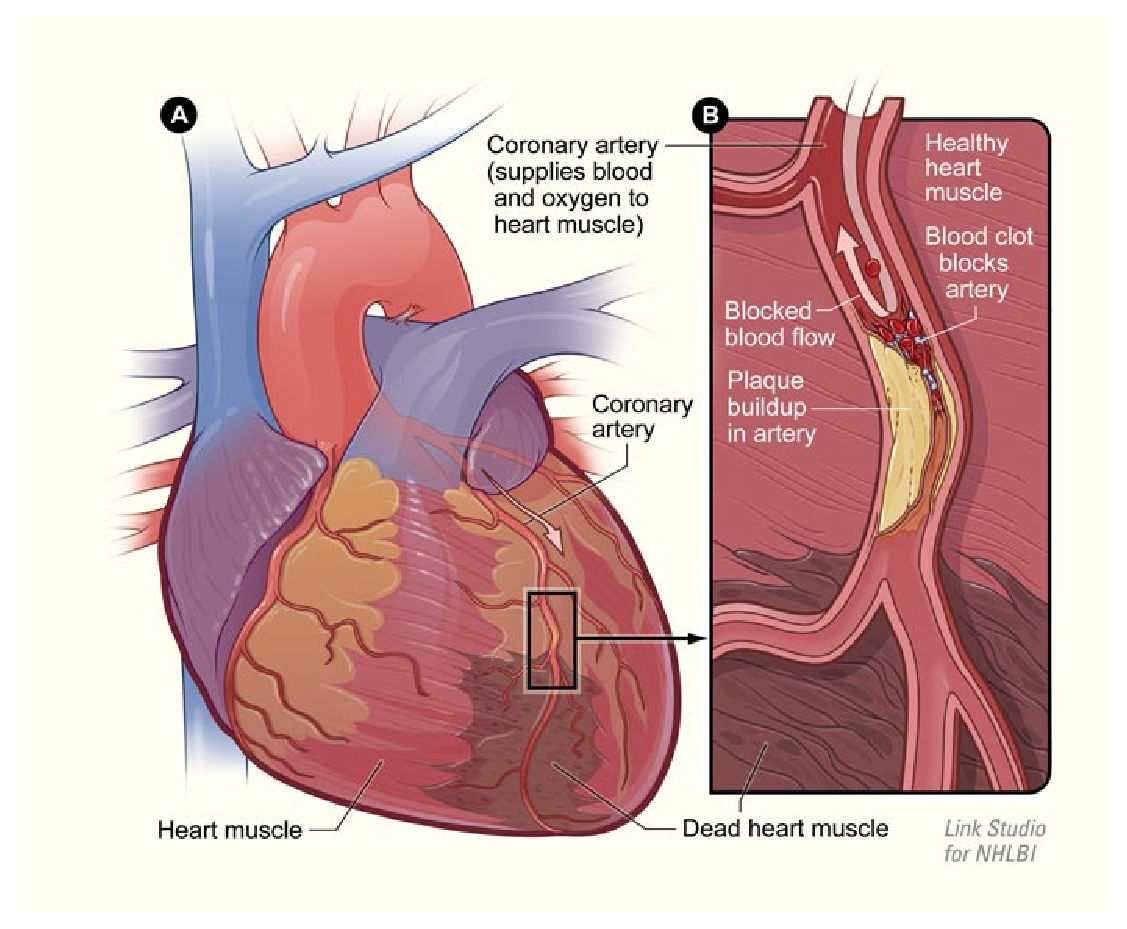
\includegraphics[height=120pt]{../../Figures/background/heart_attack_large.eps}
\caption[冠心病病理]{图片来自:\url{http://www.nhlbi.nih.gov/index.html}}
% \label{fig:heart_attack}
\end{figure}
\end{frame}

\begin{frame}
\begin{columns}[onlytextwidth]
\begin{column}{0.4\textwidth}
\begin{figure}[t]
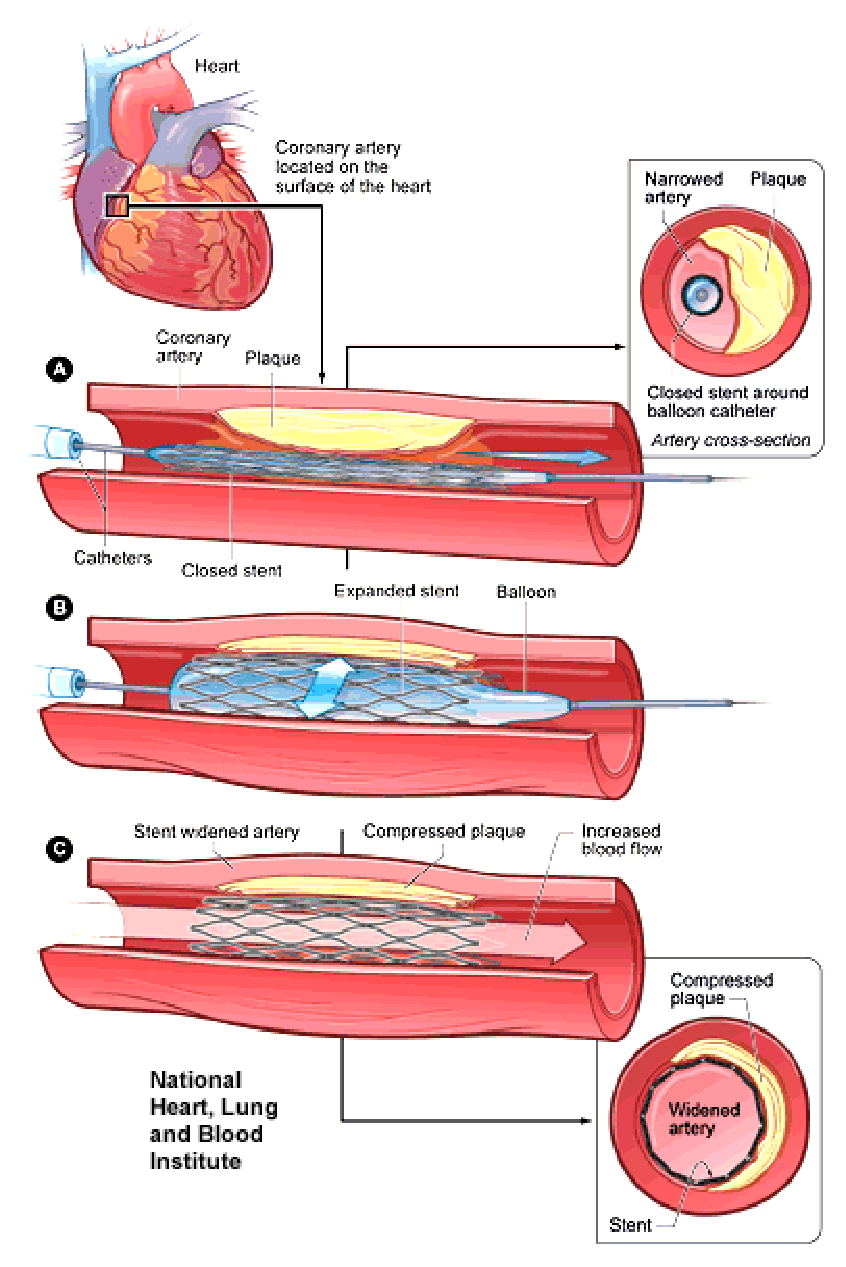
\includegraphics[height=170pt]{../../Figures/background/phauthuatmachmau_stent.eps}
\caption[冠状动脉介入术]{图片来自:\\\url{http://www.nhlbi.nih.gov/index.html}}
\end{figure}
\end{column}
\begin{column}{0.5\textwidth}
\begin{itemize}
\item \textbf{冠状动脉介入术}: 
\begin{itemize}
\item \footnotesize{重建冠脉血运的微创介入手术}
\end{itemize}
\item \textbf{主要步骤}:
\begin{enumerate}[A]
\item \footnotesize{将载有气囊的导管沿主动脉送至病灶位置}
\item \footnotesize{向气囊注入空气使其膨胀,迫使气囊外的支架扩张}
\item \footnotesize{通过导管抽出气囊内的空气使其收缩后撤出}
\end{enumerate}
\end{itemize}
\begin{itemize}
\pause \item \textbf{相较于传统手术的优势}
\begin{itemize}
% \setlength{\itemindent}{-.1in}
\item 创口微小
\item 痛苦减轻
\item 较短的手术时间
\item 并发症发生率低
\item 术后恢复快
\end{itemize}
\end{itemize}
\end{column}
\end{columns}
\end{frame}

\begin{frame}
\begin{itemize}
  \item \textbf{“师傅-学徒”模式的技艺传承}: 
  \begin{enumerate}[A]
    \item 手工技艺的传承
    \item 医学技术的传承
  \end{enumerate}
\end{itemize}
\begin{figure}
\begin{minipage}[t]{0.8\linewidth}
\centering
% top
\subfigure[]{

\includegraphics[height=60pt]{../../Figures/background/220px-Apprenticeship.eps}
\quad
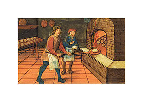
\includegraphics[height=60pt]{../../Figures/background/220px-Medieval_baker.eps}
}
% bottom
\subfigure[]{
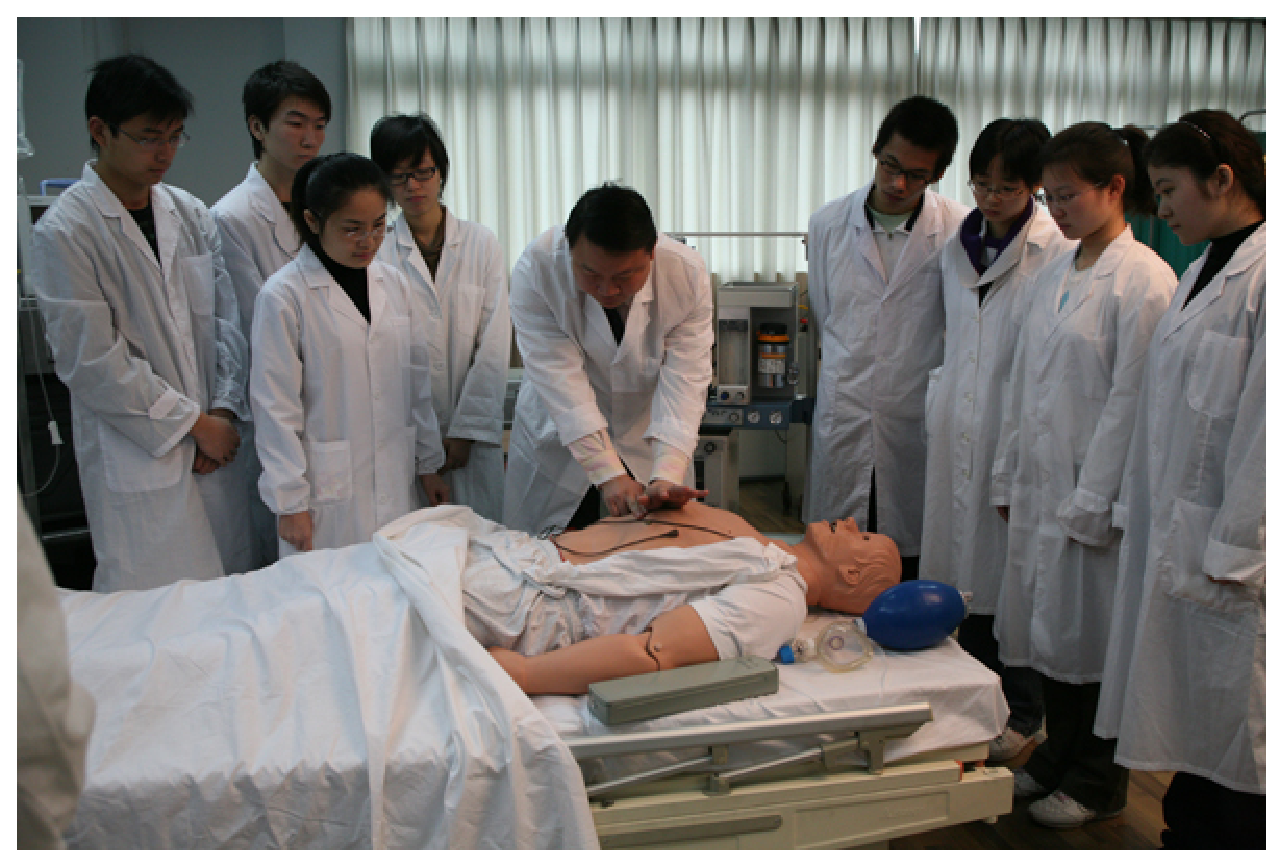
\includegraphics[height=70pt]{../../Figures/background/clinical_training_center.eps}
\quad
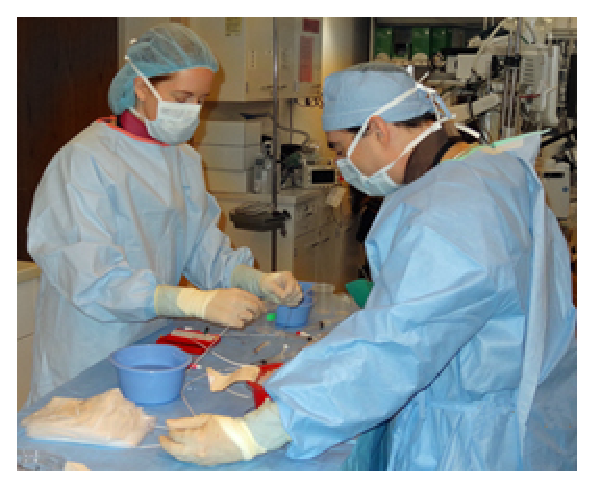
\includegraphics[height=70pt]{../../Figures/background/cath_lab.eps}
}	
\end{minipage}
\end{figure}
\end{frame}

\begin{frame}
\begin{itemize}
  \item \textbf{微创血管介入手术机器人系统~[Ji(2011)]}: 
  \begin{enumerate}
    \onslide<1-2> \item 机器人系统外观
    \onslide<2>\item 机器人控制系统
  \end{enumerate}
\end{itemize}
\begin{columns}[b,onlytextwidth]
\begin{column}{.5\textwidth}
\onslide<1-2>\begin{figure}[t]
\centering
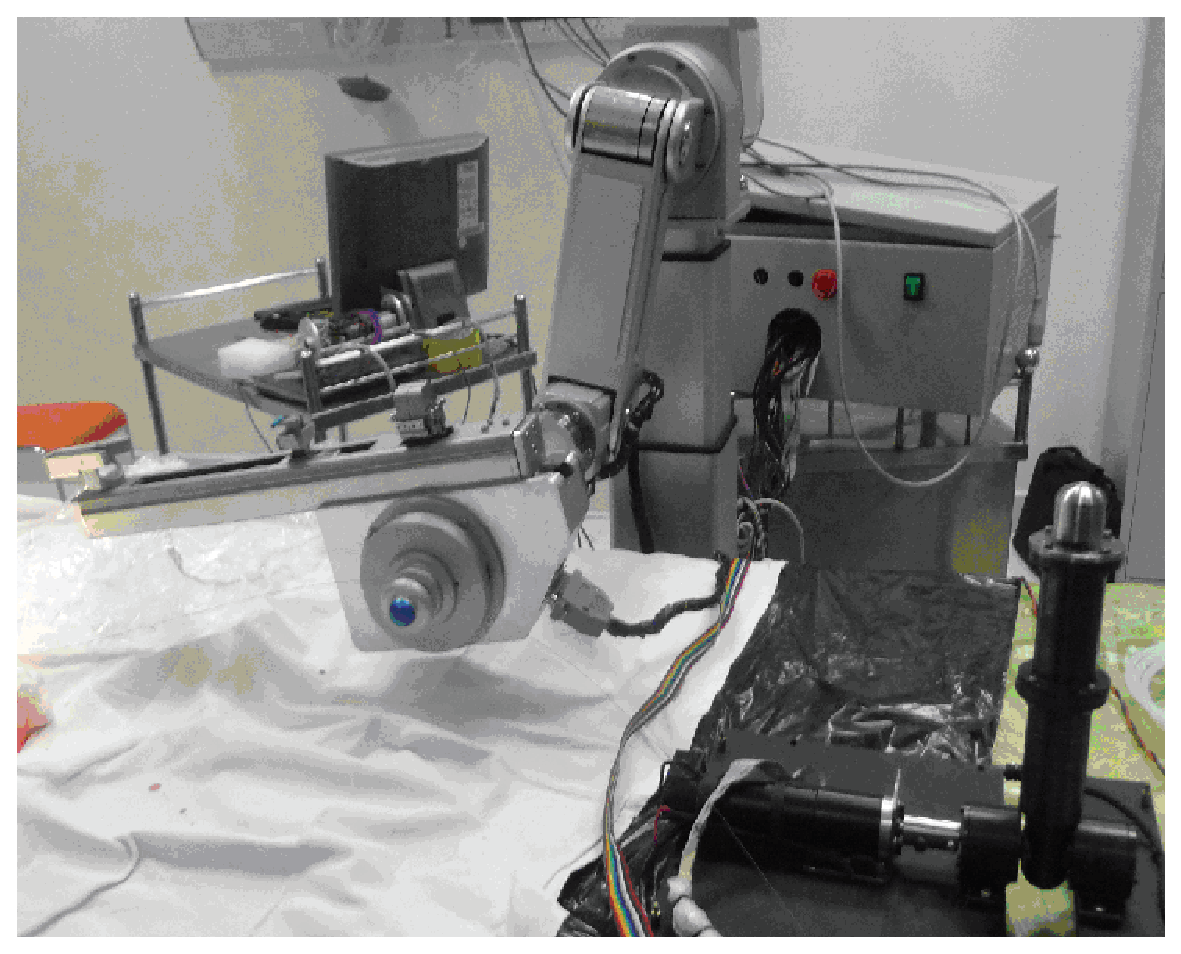
\includegraphics[height=100pt]{../../Figures/background/robot.eps}
\end{figure}
\end{column}
\begin{column}{.5\textwidth}
\onslide<2> \begin{figure}[t]
\centering
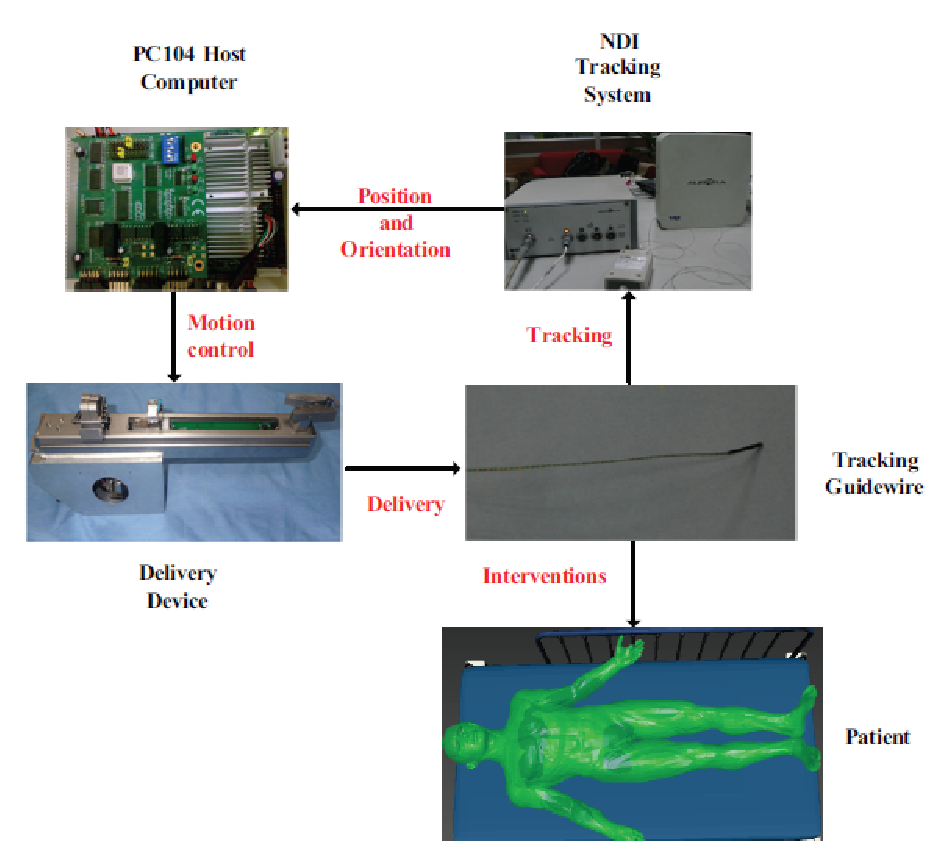
\includegraphics[height=100pt]{../../Figures/background/robot_arch.eps}
\end{figure}
\end{column}
\end{columns}
\end{frame}

\begin{frame}
\begin{itemize}
  \item \textbf{微创血管介入手术仿真系统}: 
  % \begin{enumerate}
    % \item 机器人外观
    % \item 机器人控制系统
  % \end{enumerate}
\end{itemize}
% \begin{columns}[b,onlytextwidth]
% \begin{column}{.5\textwidth}
\begin{figure}[t]
\centering
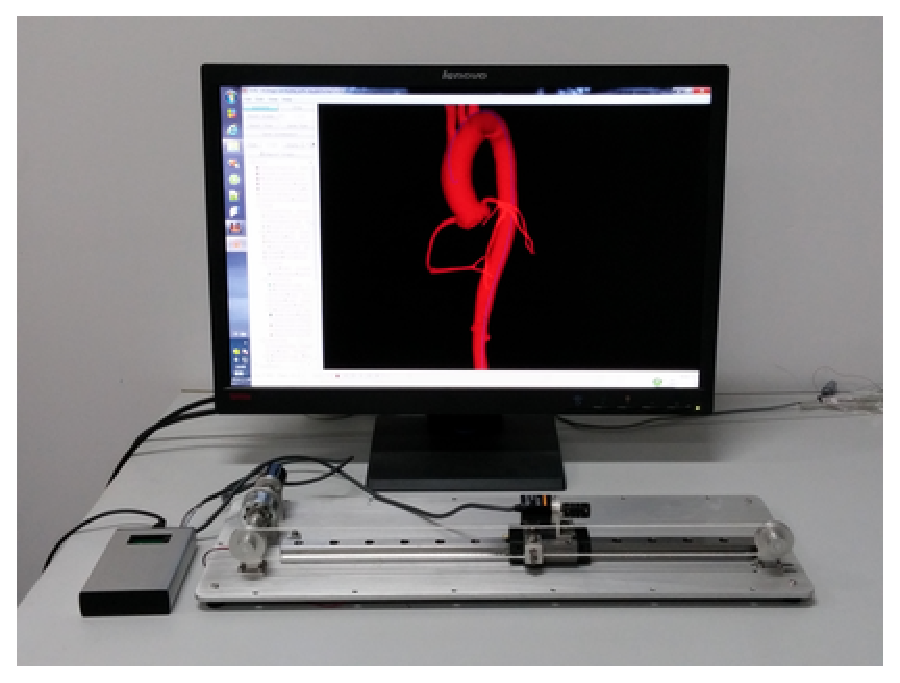
\includegraphics[height=130pt]{../../Figures/background/simulator.eps}
\end{figure}
% \end{column}
% \begin{column}{.5\textwidth}
% \begin{figure}[t]
% \centering
% \input{../../FigureSrc/background/architecture_utf8}
% \end{figure}
% \end{column}
% \end{columns}
\end{frame}

\begin{frame}
\begin{itemize}
  \item \textbf{微创血管介入手术机器人系统的主要功能}: 
  \begin{enumerate}
    \onslide<1-5> \item 虚拟解剖环境
    \onslide<2-5> \item 虚拟手术工具
    \onslide<5> \item 触觉接口装置
  \end{enumerate}
\end{itemize}
\begin{columns}[b,onlytextwidth]
\begin{column}{.25\textwidth}
\onslide<3-5> \begin{figure}[t]
\centering
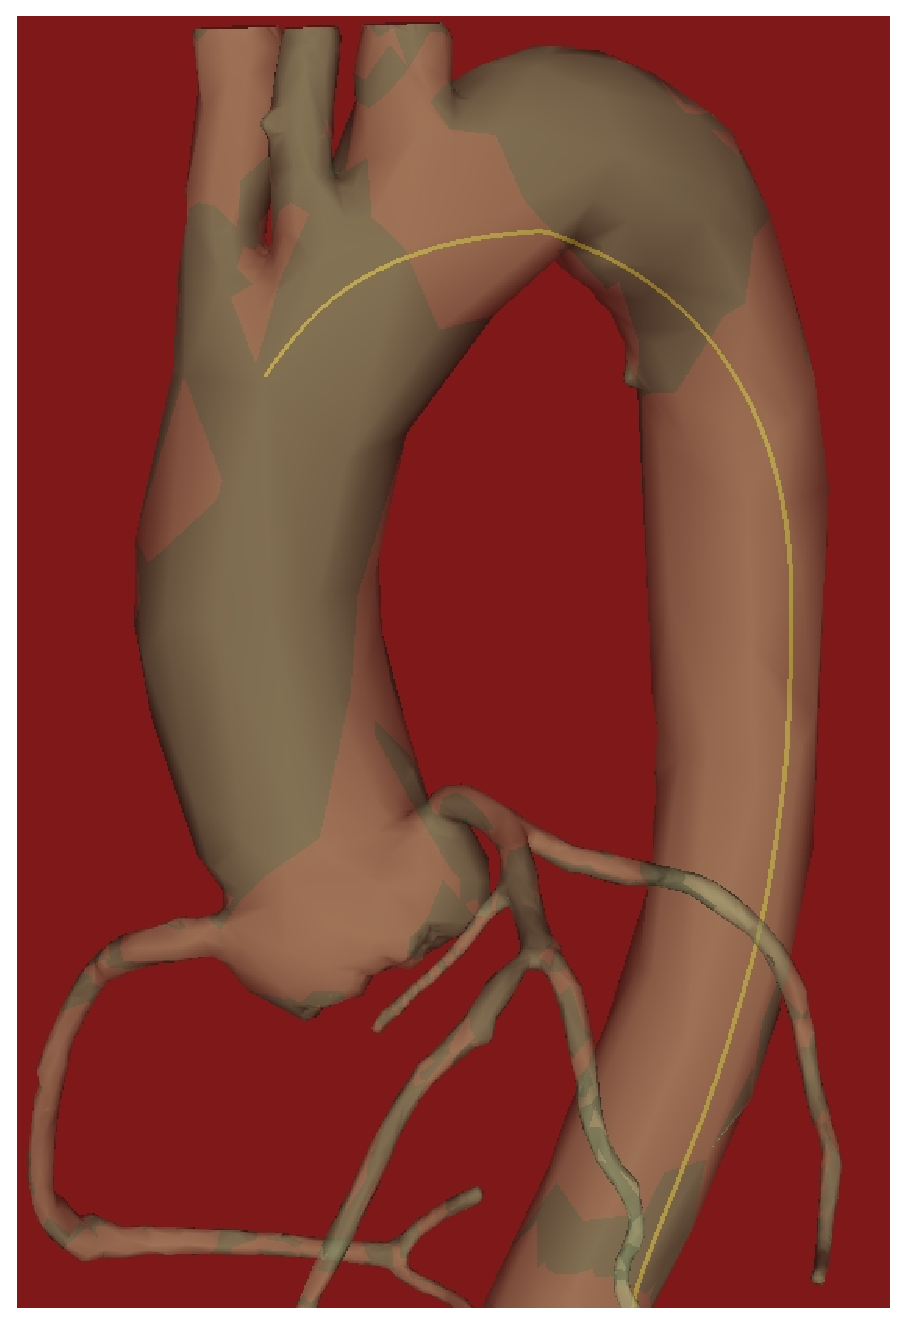
\includegraphics[height=1.0in]{../../Figures/background/simulation2.eps}
% 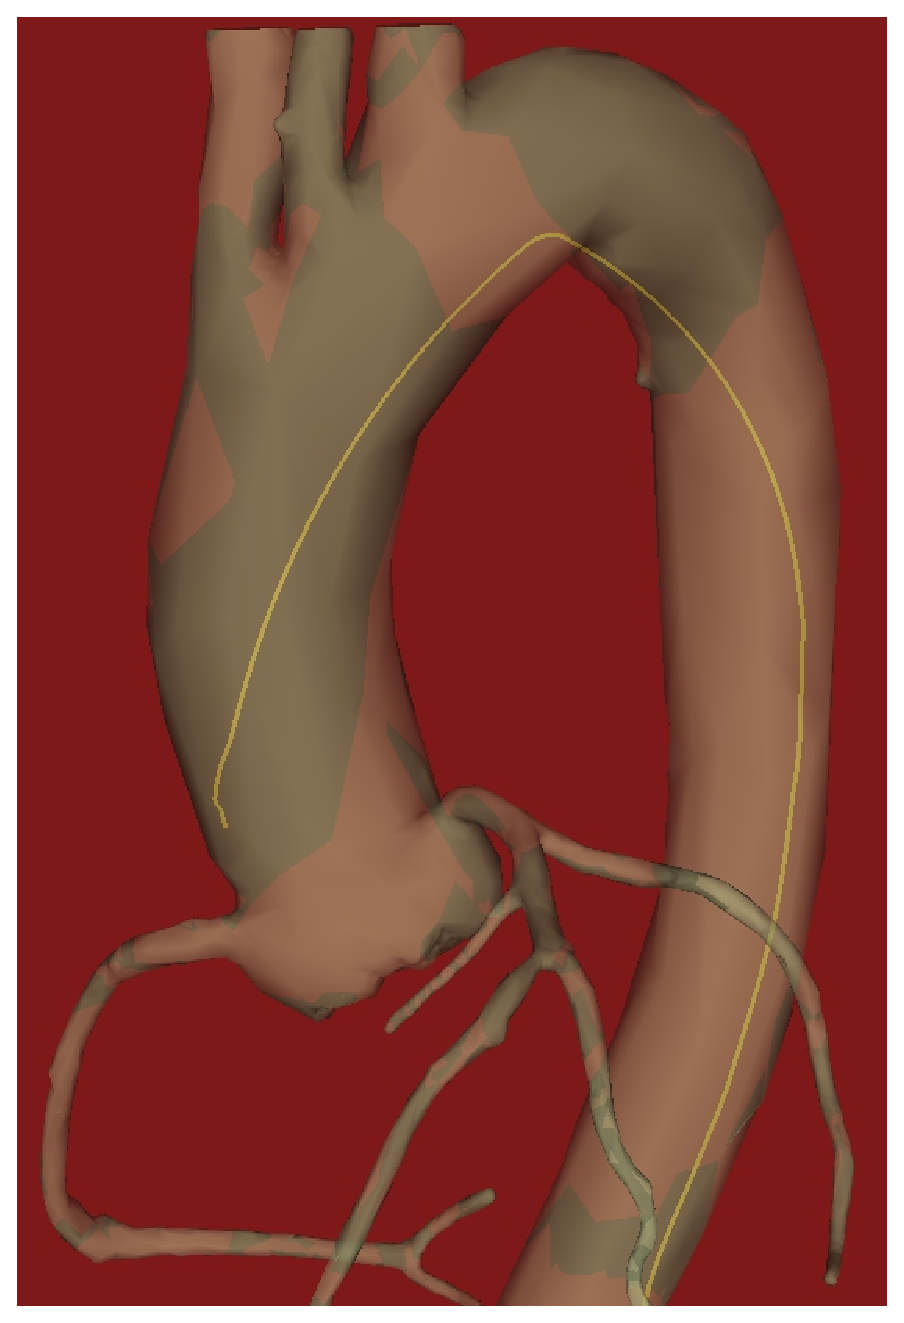
\includegraphics[height=1.0in]{../../Figures/background/simulation.eps}
% 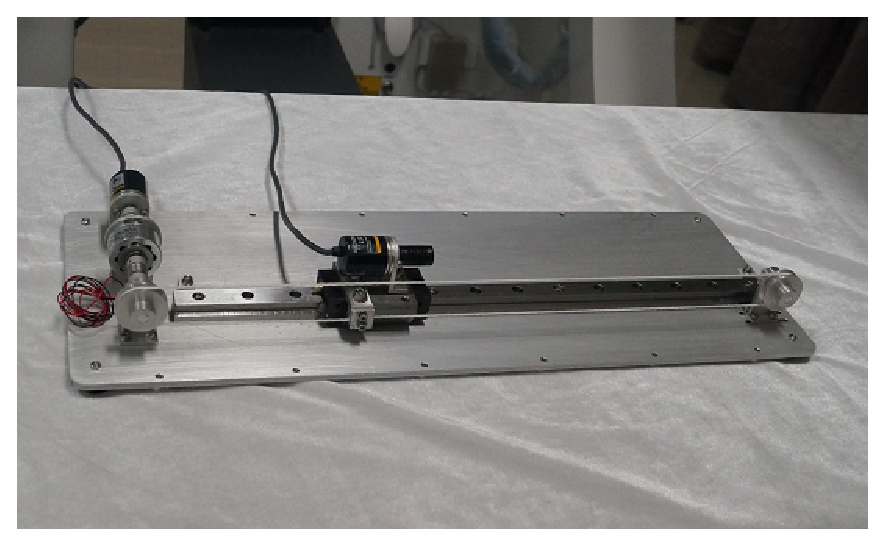
\includegraphics[height=1.0in]{../../Figures/background/interface.eps}
\end{figure}
\end{column}
\begin{column}{.25\textwidth}
\onslide<4-5> \begin{figure}[t]
\centering
% 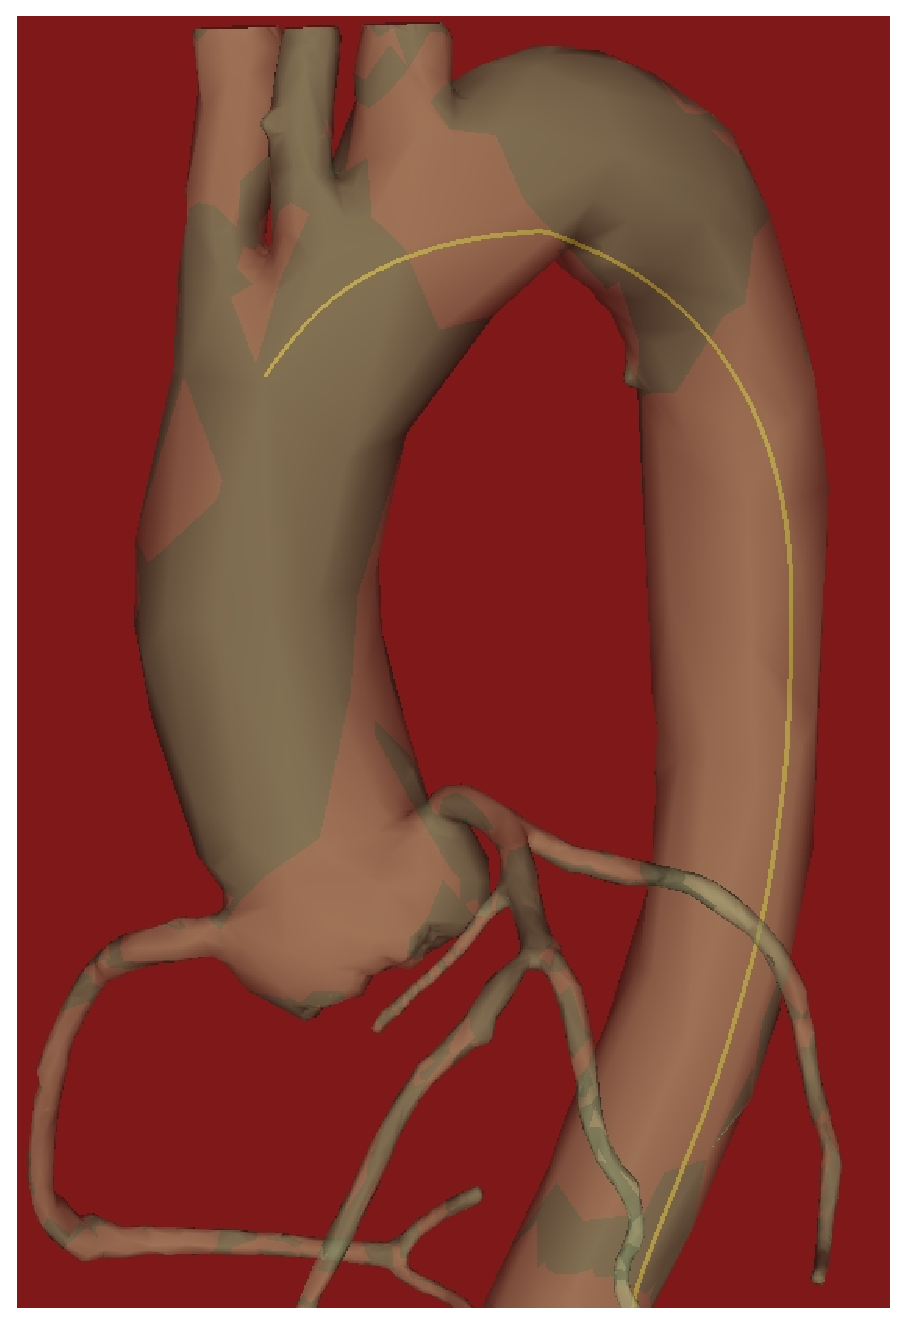
\includegraphics[height=1.0in]{../../Figures/background/simulation2.eps}
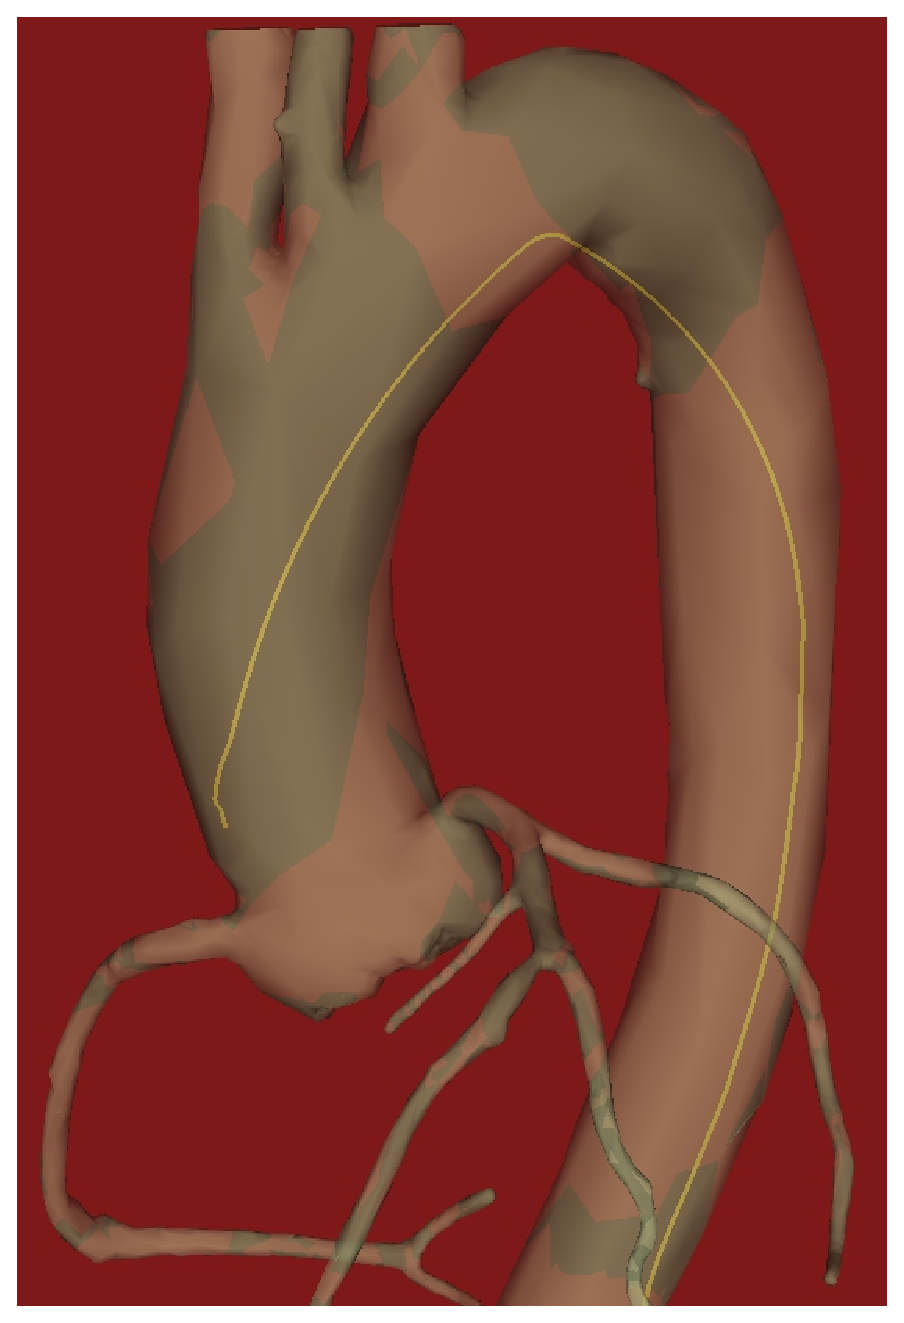
\includegraphics[height=1.0in]{../../Figures/background/simulation.eps}
% 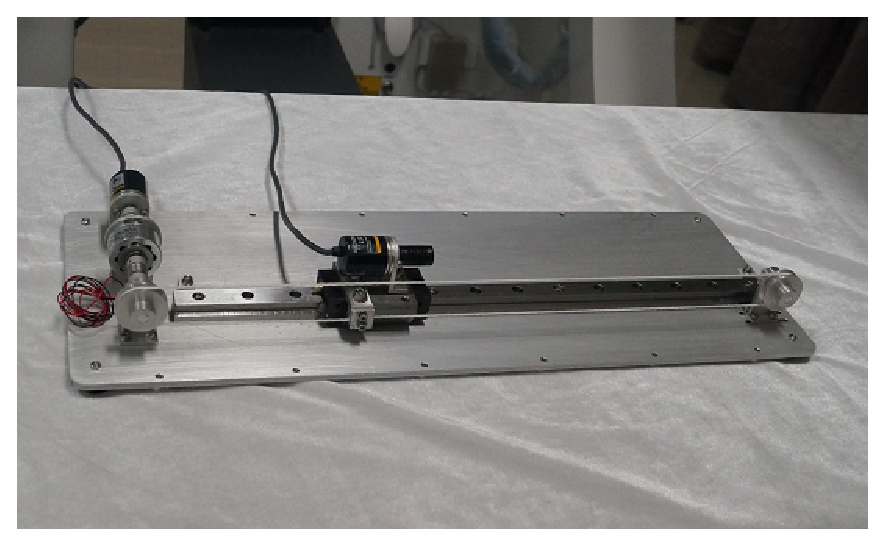
\includegraphics[height=1.0in]{../../Figures/background/interface.eps}
\end{figure}
\end{column}
\begin{column}{.5\textwidth}
\onslide<5> \begin{figure}[t]
\centering
% 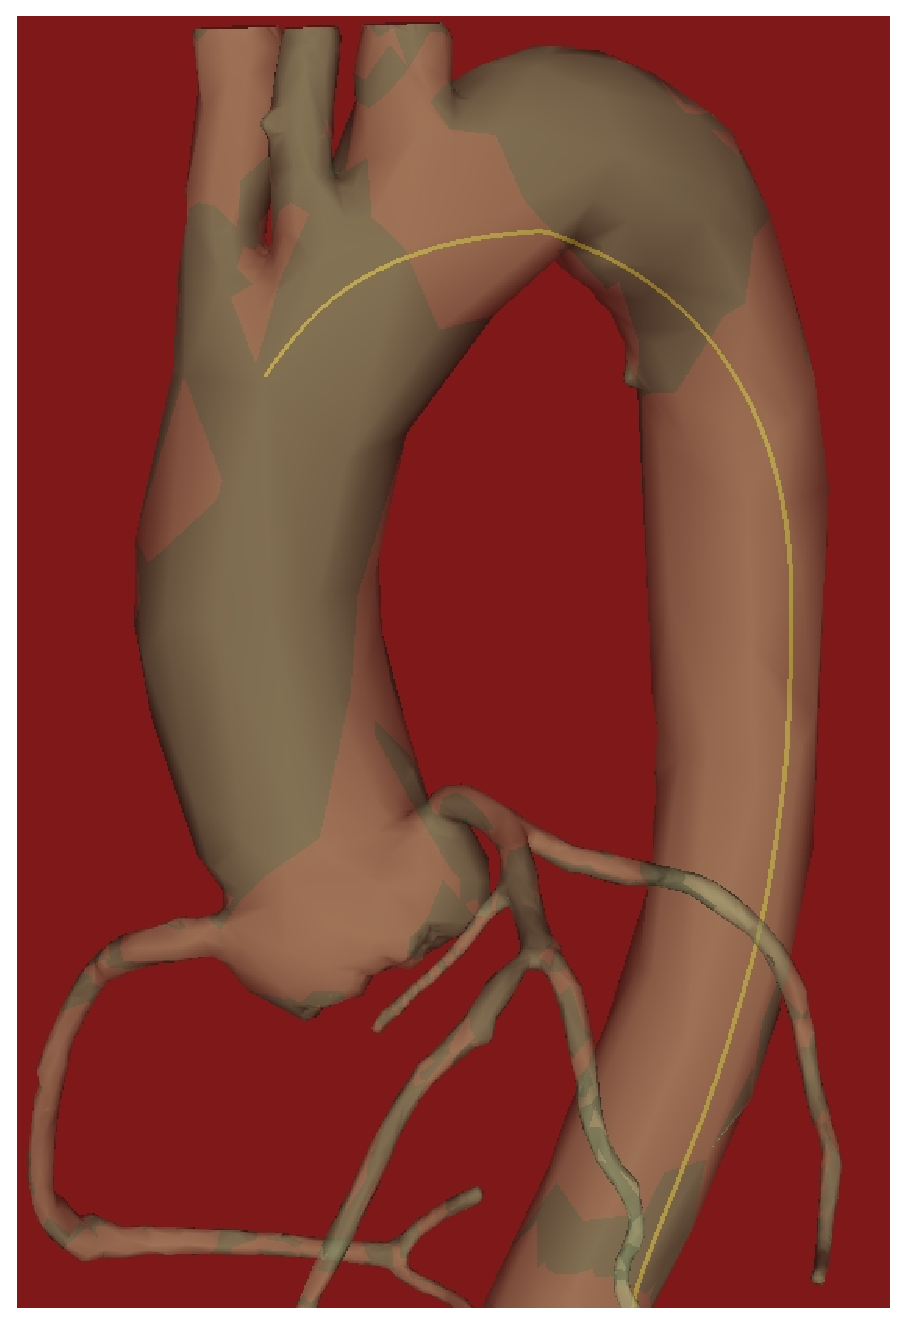
\includegraphics[height=1.0in]{../../Figures/background/simulation2.eps}
% 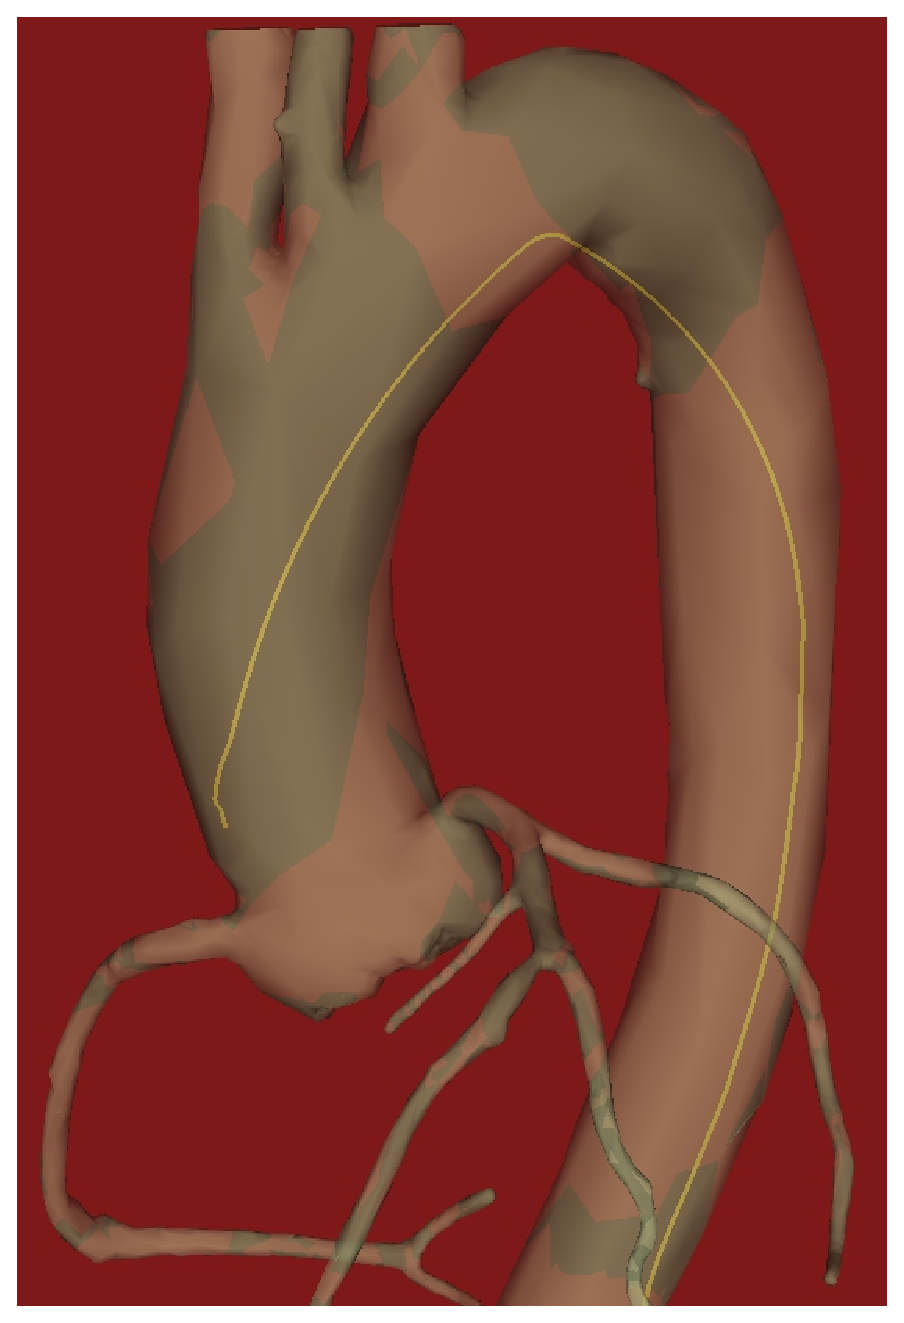
\includegraphics[height=1.0in]{../../Figures/background/simulation.eps}
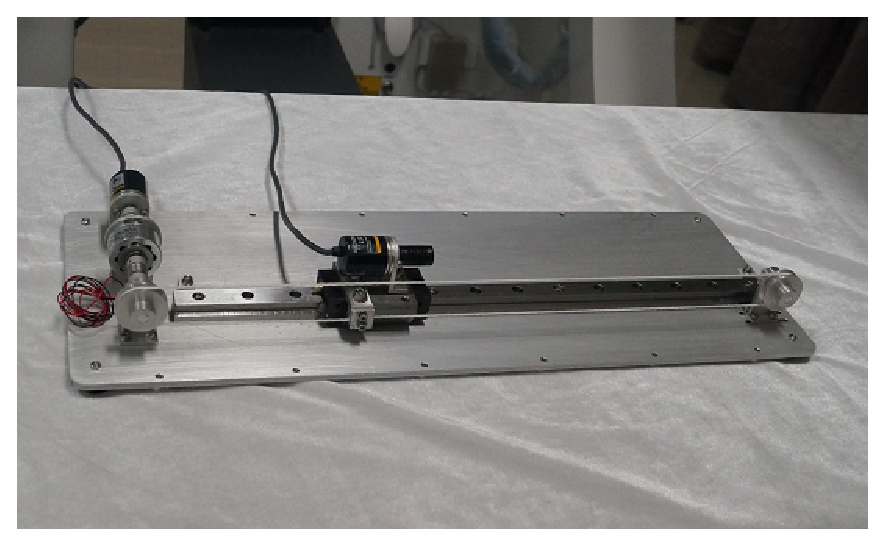
\includegraphics[height=1.0in]{../../Figures/background/interface.eps}
\end{figure}
\end{column}
\end{columns}
\end{frame}

\begin{frame}
\begin{itemize}
\item \textbf{技术难点}
\begin{itemize}
\pause \item 影像中主动脉与脊椎间隙过小甚至接触
\pause \item 影像中冠状动脉的亮度较暗,且走向多变,直径较小
\pause \item 心脏搏动导致心脏区域成像效果较差,无法准确提取完整模型
\pause \item 重建的表面模型数据量大,影响交互仿真
\pause \item 重建的表面模型数据量大,难以进行几何信息提取运算
\end{itemize}
\end{itemize}
\end{frame}

\begin{frame}
\begin{itemize}
  \item \textbf{本文贡献}
  \begin{itemize}
    \onslide<1-3> \item \textbf{基于真实病例数据的人心血管模型的创建}
    \begin{itemize}
      \onslide<2-3> \item 提出创建主动脉内腔模型的方法
      \onslide<2-3> \item 提出创建冠状动脉主要分支模型的方法
      \onslide<2-3> \item 提出创建冠状动脉次级分支模型的方法
      \onslide<2-3> \item 提出创建心脏近似模型的方法
    \end{itemize}
    \onslide<1-3> \item \textbf{面向交互仿真的人心血管模型的后处理}
    \begin{itemize}
      \onslide<3> \item 提出面向交互仿真的模型优化方法
      \onslide<3> \item 提出面向虚拟训练的模型几何信息提取方法
    \end{itemize}
  \end{itemize}
\end{itemize}
\end{frame} 
\section{医学影像处理}
%# -*- coding:utf-8 -*-
\subsection[主动脉分割]{基于测地活动轮廓的主动脉分割}

\begin{frame}
\begin{itemize}
\item \textbf{血管介入仿真中主动脉模型的作用}
\begin{itemize}
\item 可视化环境的组成部分
\item 虚拟导管运动的必经路径
\item 虚拟导管交互的硬约束
\end{itemize}
\pause \item \textbf{血管介入仿真中主动脉模型的获取}
\begin{itemize}
\item 几何形状近似的中空管道
\item 逐帧手动提取主动脉区域
\item 医学影像处理方式
\end{itemize}
\pause \item \textbf{主动脉内腔的分割与可视化}
\begin{itemize}
\item 仍是医学影像领域中一项具有挑战性的工作
\item 主动脉形态特点:走向稳定,截面大小变化均匀
\item 分割时的主要困难:与骨骼以及腹腔内脏器有交叠,影响分割
\end{itemize}
\end{itemize}
\end{frame} 

\begin{frame}
\begin{itemize}
\item \textbf{测地活动轮廓(GAC)~[Caselles(1997)]}
\begin{itemize}
\pause \item 根植于“蛇”模型
\begin{itemize}
\item 基于图像内容呈现的物理性质,通过演进一个轮廓(或“围线”),探测物体边缘
\item 演进通过使一个能量泛函最小化来实现,取得(局部)最小值的位置恰好是目标物体的边缘
\item \textbf{“蛇”的缺点}:轮廓无法控制自身拓扑;无法同时探测多个目标
\end{itemize}
\pause \item 对“蛇”模型的改进
\begin{itemize}
\item 引入测地学计算和水平集演进
\item 允许围线同时探测图像中多个目标的内部边缘和外部边缘
\end{itemize}
\end{itemize}
\end{itemize}
\end{frame}

\begin{frame}
\begin{itemize}
\onslide<1-2> \item \textbf{经典“蛇”模型}
\begin{equation*}
% \label{eqn:aorta_particular_snakes}
E(\mathcal{C}) = \alpha \int_0^1 | \mathcal{C}'(q) |^2 dq + \beta \int_0^1 | \mathcal{C}''(q) |^2 dq - \lambda \int_0^1 | \nabla I_{s} ( \mathcal{C}(q) ) |dq
\end{equation*}
\onslide<2>  \item \textbf{GAC的数学模型}
% \end{itemize}
\begin{equation*}
% \label{eqn:aorta_particular_snakes}
E(\mathcal{C}) = \alpha \int_0^1 | \mathcal{C}'(q) |^2 dq - \lambda \int_0^1 | \nabla I_{s} ( \mathcal{C}(q) ) |dq
\end{equation*}
% \quad\quad其中:
\onslide<1-2> \begin{itemize}
\item $E(\cdot)$:能量泛函
\item $\mathcal{C}(\cdot)$:参数化平面内曲线
\item $I_{s}(\cdot)$:含有待探测目标的图像
\item $\alpha$:传导常数
\item $\beta$:扩散常数
\item $\lambda$:曲率常数
\end{itemize}
\end{itemize}
\end{frame}

\begin{frame}
\begin{itemize}
\onslide<1-3> \item \textbf{围线演进的光学比拟}:光学中的Fermat原理
\begin{equation*}
L_{R} = \int_{A}^{B} n(s) ds
\end{equation*}
\begin{itemize}
\item $L_{R}$:光线在介质中的传播路径的弧长
\item $A$,$B$:传播路径的起点和终点
\item $n(\cdot)$:介值的折射率
\end{itemize}
\onslide<2-3> \item \textbf{Fermat原理的结论:在传播过程中,路径不是直线,而是按最短光程的方式来确定}
\onslide<3> \item \textbf{GAC模型:在界面演进过程中,使能量$E$达到局部最小}
\end{itemize}
\end{frame}

\begin{frame}
\begin{itemize}
\onslide<1-2> \item \textbf{围线演进目标}
\begin{equation*}
\min \int_0^1 g(|\nabla I_{s} ( \mathcal{C} (q) )|) |\mathcal{C}' (q)| dq
\end{equation*}
\begin{itemize}
\item $g(\cdot)$等同于曲线演进速度,依赖细节几何性质,独立于测地计算
\end{itemize}
\onslide<2> \item \textbf{基于特征图像的演进目标}
\begin{equation*}
\min \int_0^1 g(\nabla I_{\sigma}) |\mathcal{C}' (q)| dq
\end{equation*}
\begin{itemize}
\item $I_{\sigma}$:源图像的特征图像
\end{itemize}
\end{itemize}
\end{frame}

\begin{frame}
\begin{itemize}
\onslide<1-2> \item \textbf{围线演进方程}:下式左边为零时,围线演进至目标边缘
\begin{equation*}
\label{eqn:EvolutionModel}
\frac{\partial \mathcal{C}(t)}{\partial t} = g(I_{\sigma}) \kappa \mathcal{N} - (\nabla g(I_{\sigma}) \cdot \mathcal{N}) \mathcal{N}
\end{equation*}
\begin{itemize}
\item $\kappa$:曲线$\mathcal{C}$的曲率
\item $\mathcal{N}$:指向曲线$\mathcal{C}$“内部”的单位法向量
\item 两种“力”的作用:第一项是内力(形变力);第二项是外力(向边界移动)
\end{itemize}
\onslide<2> \item \textbf{围线更新方程}:围线的演进等同于其嵌入水平集$u$的更新
\begin{equation*}
\frac{\partial u}{\partial t} = g(I_{\sigma}) |\nabla u| \kappa + \nabla g(I_{\sigma}) \cdot \nabla u
\end{equation*}
\end{itemize}
\end{frame}

\begin{frame}
\begin{itemize}
\item \textbf{主动脉内腔分割流程}
\end{itemize}
\begin{figure}[t]
\centering
%# -*- coding:utf-8 -*-
\begin{tikzpicture}[scale=.37]

\draw [black,thick,rounded corners] (-3,0) rectangle (3,2);            % binary threshold
\draw [black,thick,rounded corners] (-3,3) rectangle (3,5);  % CURVES

\draw [black,thick,rounded corners] (-8,7) rectangle (-2,9);   % initial contours

\draw [black,thick,rounded corners] (2,7) rectangle (8,9);     % feature images

\draw [black,thick,rounded corners] (-3,11) rectangle (3,13);  % thresholding
\draw [black,thick,rounded corners] (-3,14) rectangle (3,16);  % curvature anisotropic diffusion
\draw [black,thick,rounded corners] (-3,17) rectangle (3,19);  % raw input

\node [above right] at (-2.25,0.25) {\scriptsize \fs \bf 二值阈值滤波};
\node [above right] at (-2.25,3.25) {\scriptsize \fs \bf 测地活动轮廓};

\node [above right] at (-7.65,7.35) {\scriptsize \fs \bf 初始水平集演进};

\node [above right] at (2.82,7.35) {\scriptsize \fs \bf 特征图像计算};

\node [above right] at (-2.3,11.35) {\scriptsize \fs \bf 二值阈值滤波};
\node [above right] at (-2.9,14.35) {\scriptsize \fs \bf 曲率各向异性扩散};
\node [above right] at (-1.95,17.35) {\scriptsize \fs \bf ROI体数据};

\draw [<-,thick] (0,2) -- (0,3);

\draw [<-,thick] (0,5) -- (0,6);
\draw [thick] (-5,6) -- (5,6);
\draw [thick] (-5,6) -- (-5,7);
\draw [thick] (5,6) -- (5,7);

\draw [<-,thick] (-5,9) -- (-5,10);
\draw [<-,thick] (5,9) -- (5,10);
\draw [thick] (-5,10) -- (5,10);
\draw [thick] (0,10) -- (0,11);

\draw [<-,thick] (0,13) -- (0,14);
\draw [<-,thick] (0,16) -- (0,17);

\end{tikzpicture} 
% 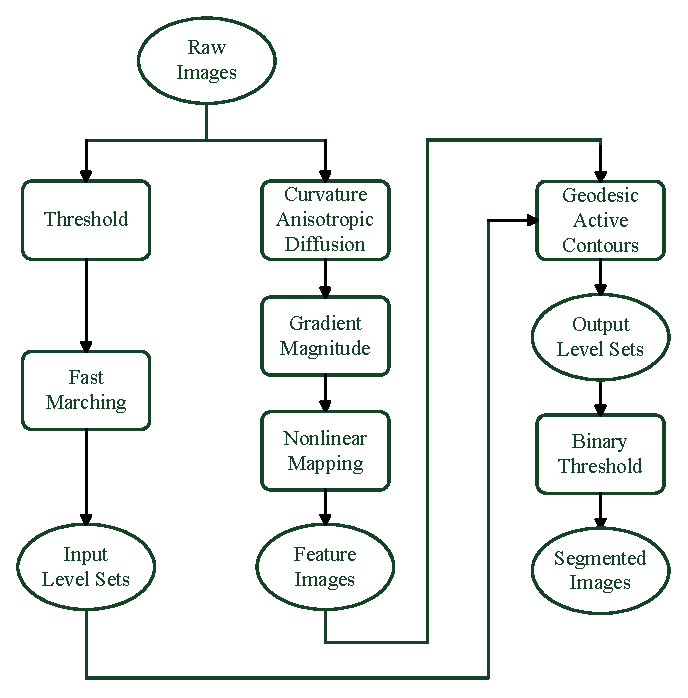
\includegraphics[width=3.2in]{Figures/gac/DataFlow.eps}
% \caption[主动脉内腔分割流程]{主动脉内腔分割流程。}
% \label{fig:aorta_data_flow}
\end{figure}
\end{frame}

\begin{frame}
\begin{itemize}
\item \textbf{原始图像的ROI提取}
\begin{itemize}
\pause \item 设定矩形区域的起点和尺寸
\pause \item 缩小处理区域,减轻运算负担
\end{itemize}
\end{itemize}
\begin{figure}[t]
\centering
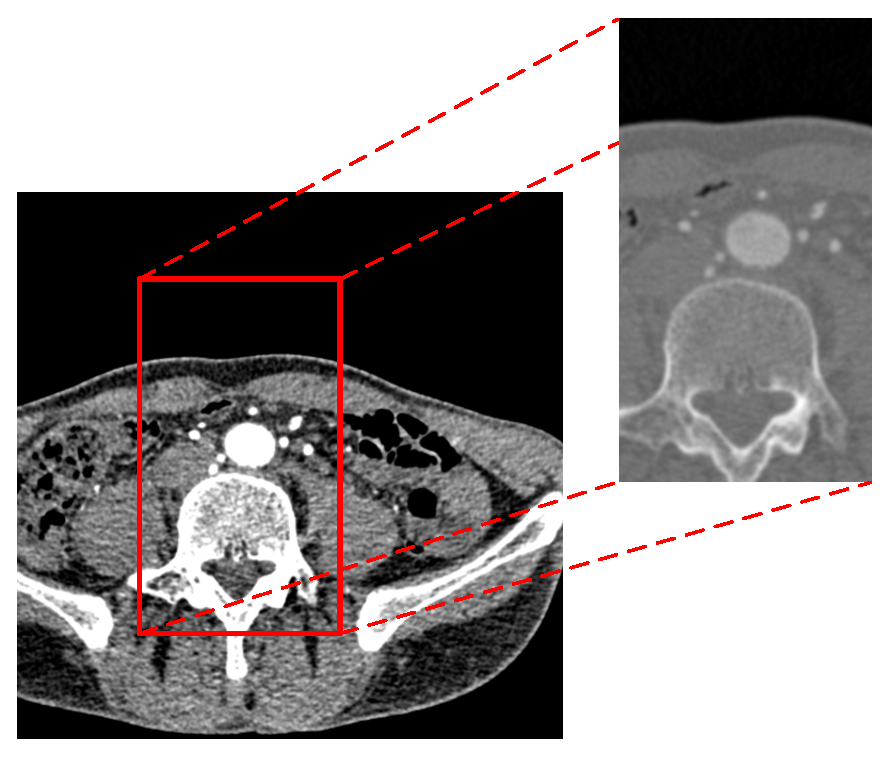
\includegraphics[width=2.0in]{../../Figures/gac/ROI.eps}
% \caption[原始图像的ROI提取]{原始图像的ROI提取。}
% \label{fig:aorta_roi}
\end{figure}
\end{frame}

\begin{frame}
\begin{itemize}
  \item \textbf{特征图像的生成步骤}:
  \begin{enumerate}
    \onslide<1-3> \item 保护物体边缘的平滑处理(曲率各向异性扩散滤波,$\text{传导参数} = 9.0$)
    \onslide<2-3> \item 梯度幅值计算(基于Gaussian核,$\sigma = 0.9$)
    \onslide<3> \item 像素亮度非线性映射(S型函数,$m = -3$, $n = 20$)
  \end{enumerate}
\end{itemize}
\begin{columns}[b,onlytextwidth]
\begin{column}{.3\textwidth}
\onslide<1-3> \begin{figure}[t]
\centering
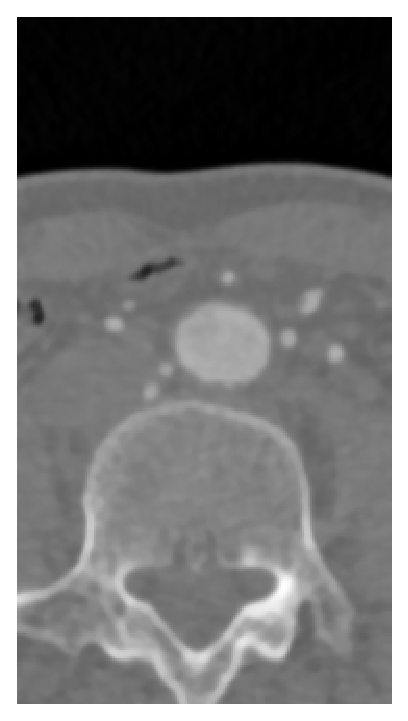
\includegraphics[height=1.5in]{../../Figures/gac/dcm_smoothing.eps}
\end{figure}
\end{column}
\begin{column}{.3\textwidth}
\onslide<2-3> \begin{figure}[t]
\centering
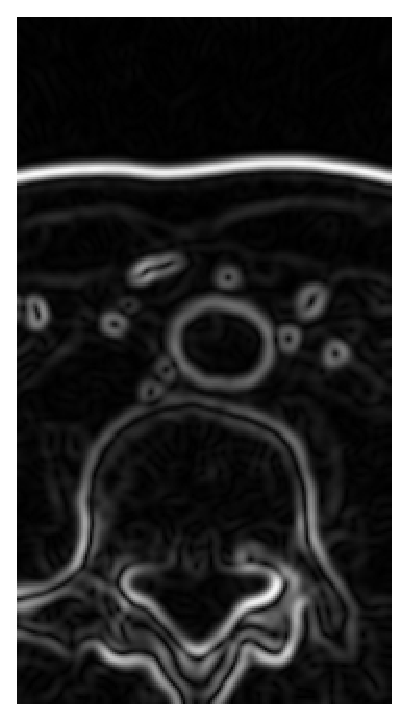
\includegraphics[height=1.5in]{../../Figures/gac/dcm_gradient.eps}
\end{figure}
\end{column}
\begin{column}{.3\textwidth}
\onslide<3> \begin{figure}[t]
\centering
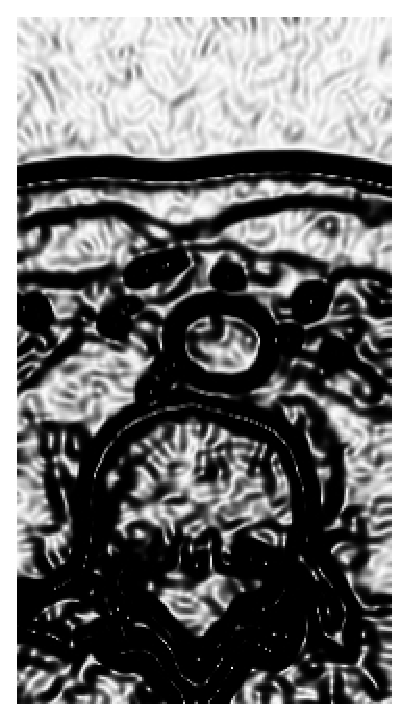
\includegraphics[height=1.5in]{../../Figures/gac/dcm_sigmoid.eps}
\end{figure}
\end{column}
\end{columns}
\end{frame}

\begin{frame}
\begin{itemize}
  \item \textbf{水平集演进过程}:
  \begin{enumerate}
    \onslide<1-4> \item 阈值滤波($\text{TH}_{\text{lower}} = 300\text{HU}$, $\text{TH}_{\text{upper}} = 2000\text{HU}$)
    \onslide<2-4> \item 从某一种子点开始,利用快速步进法进行的初始水平集演进
    \onslide<3-4> \item 利用测地活动轮廓进行边缘检测(迭代次数: $100$)
    \onslide<4>  \item 利用二值阈值滤波完成像素亮度的反转(明亮区域的亮度值: $255$, 黑暗区域的亮度值: $0$)
  \end{enumerate}
\end{itemize}
\begin{columns}[b,onlytextwidth]
\begin{column}{.25\textwidth}
\onslide<1-4> \begin{figure}[t]
\centering

\includegraphics[height=1.5in]{../../Figures/gac/dcm_threshold.eps}
\end{figure}
\end{column}
\begin{column}{.25\textwidth}
\onslide<2-4> \begin{figure}[t]
\centering
\setlength{\fboxrule}{0.1pt}
\setlength{\fboxsep}{0cm}
\fbox{
\includegraphics[height=1.5in]{../../Figures/gac/dcm_fastMarching.eps}}
\end{figure}
\end{column}
\begin{column}{.25\textwidth}
\onslide<3-4> \begin{figure}[t]
\centering
\setlength{\fboxrule}{0.1pt}
\setlength{\fboxsep}{0cm}
\fbox{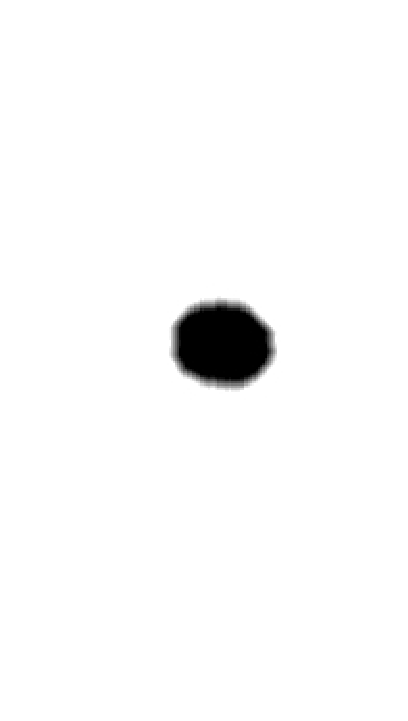
\includegraphics[height=1.5in]{../../Figures/gac/dcm_geodesic.eps}}
\end{figure}
\end{column}
\begin{column}{.25\textwidth}
\onslide<4> \begin{figure}[t]
\centering

\includegraphics[height=1.5in]{../../Figures/gac/dcm_out.eps}
\end{figure}
\end{column}
\end{columns}
\end{frame} 

\begin{frame}
\begin{itemize}
  \item \textbf{主动脉内腔分割结果评估(11组体数据)}:
  % \begin{enumerate}
    % \item 基于Jaccard系数
    % \item 基于Dice系数
  % \end{enumerate}
\end{itemize}
\begin{table}[t]
\renewcommand{\arraystretch}{0.5}
% \caption[主动脉内腔分割结果评估]{主动脉内腔表面模型分割结果评估}
% \label{tbl:aorta_evaluation}
\centering
\begin{tabular*}{70mm}{c c c}
\toprule
\hspace{2mm} \small{数据集序号}  & \hspace{2mm} \small{Jaccard}    & \hspace{2mm} \small{Dice}       \\
\midrule
\hspace{2mm} \small{1}           & \hspace{2mm} \small{$0.936434$} & \hspace{2mm} \small{$0.967174$} \\
\midrule
\hspace{2mm} \small{2}           & \hspace{2mm} \small{$0.928468$} & \hspace{2mm} \small{$0.962907$} \\
\midrule
\hspace{2mm} \small{3}           & \hspace{2mm} \small{$0.911307$} & \hspace{2mm} \small{$0.953595$} \\
\midrule
\hspace{2mm} \small{4}           & \hspace{2mm} \small{$0.918612$} & \hspace{2mm} \small{$0.957580$} \\
\midrule
\hspace{2mm} \small{5}           & \hspace{2mm} \small{$0.893099$} & \hspace{2mm} \small{$0.943531$} \\
\midrule
\hspace{2mm} \small{6}           & \hspace{2mm} \small{$0.953753$} & \hspace{2mm} \small{$0.976329$} \\
\midrule
\hspace{2mm} \small{7}           & \hspace{2mm} \small{$0.983812$} & \hspace{2mm} \small{$0.991840$} \\
\midrule
\hspace{2mm} \small{8}           & \hspace{2mm} \small{$0.922035$} & \hspace{2mm} \small{$0.959436$} \\
\midrule
\hspace{2mm} \small{9}           & \hspace{2mm} \small{$0.928791$} & \hspace{2mm} \small{$0.963081$} \\
\midrule
\hspace{2mm} \small{10}          & \hspace{2mm} \small{$0.937794$} & \hspace{2mm} \small{$0.967899$} \\
\midrule
\hspace{2mm} \small{11}          & \hspace{2mm} \small{$0.950207$} & \hspace{2mm} \small{$0.974468$} \\
\bottomrule
\end{tabular*}
\end{table}
\end{frame} 

% \begin{frame}
% \begin{itemize}
  % \item \textbf{主动脉内腔分割结果评估}:
  % \begin{enumerate}
    % \pause \item Jaccard系数
    % \pause \item Dice系数
  % \end{enumerate}
% \begin{figure}[t]
% \centering
% \input{../../FigureSrc/gac/index_utf8}
% \end{figure}
% \end{itemize}
% \end{frame}

\begin{frame}
\begin{itemize}
  \item \textbf{主动脉内腔分割结果评估}:
  \begin{enumerate}
    \onslide<1-4> \item 基于Jaccard系数(均值为$0.933$,标准差为$0.0240$)
	\begin{itemize}
	\onslide<2-4> \item 交集占并集的比重
	\end{itemize}
    \onslide<3-4> \item 基于Dice系数(均值为$0.965$,标准差为$0.0128$)
	\begin{itemize}
	\onslide<4> \item 交集占和平均的比重
	\end{itemize}
  \end{enumerate}
\end{itemize}
\begin{columns}[b,onlytextwidth]
\begin{column}{.5\textwidth}
\onslide<1-4> \begin{figure}[t]
\centering
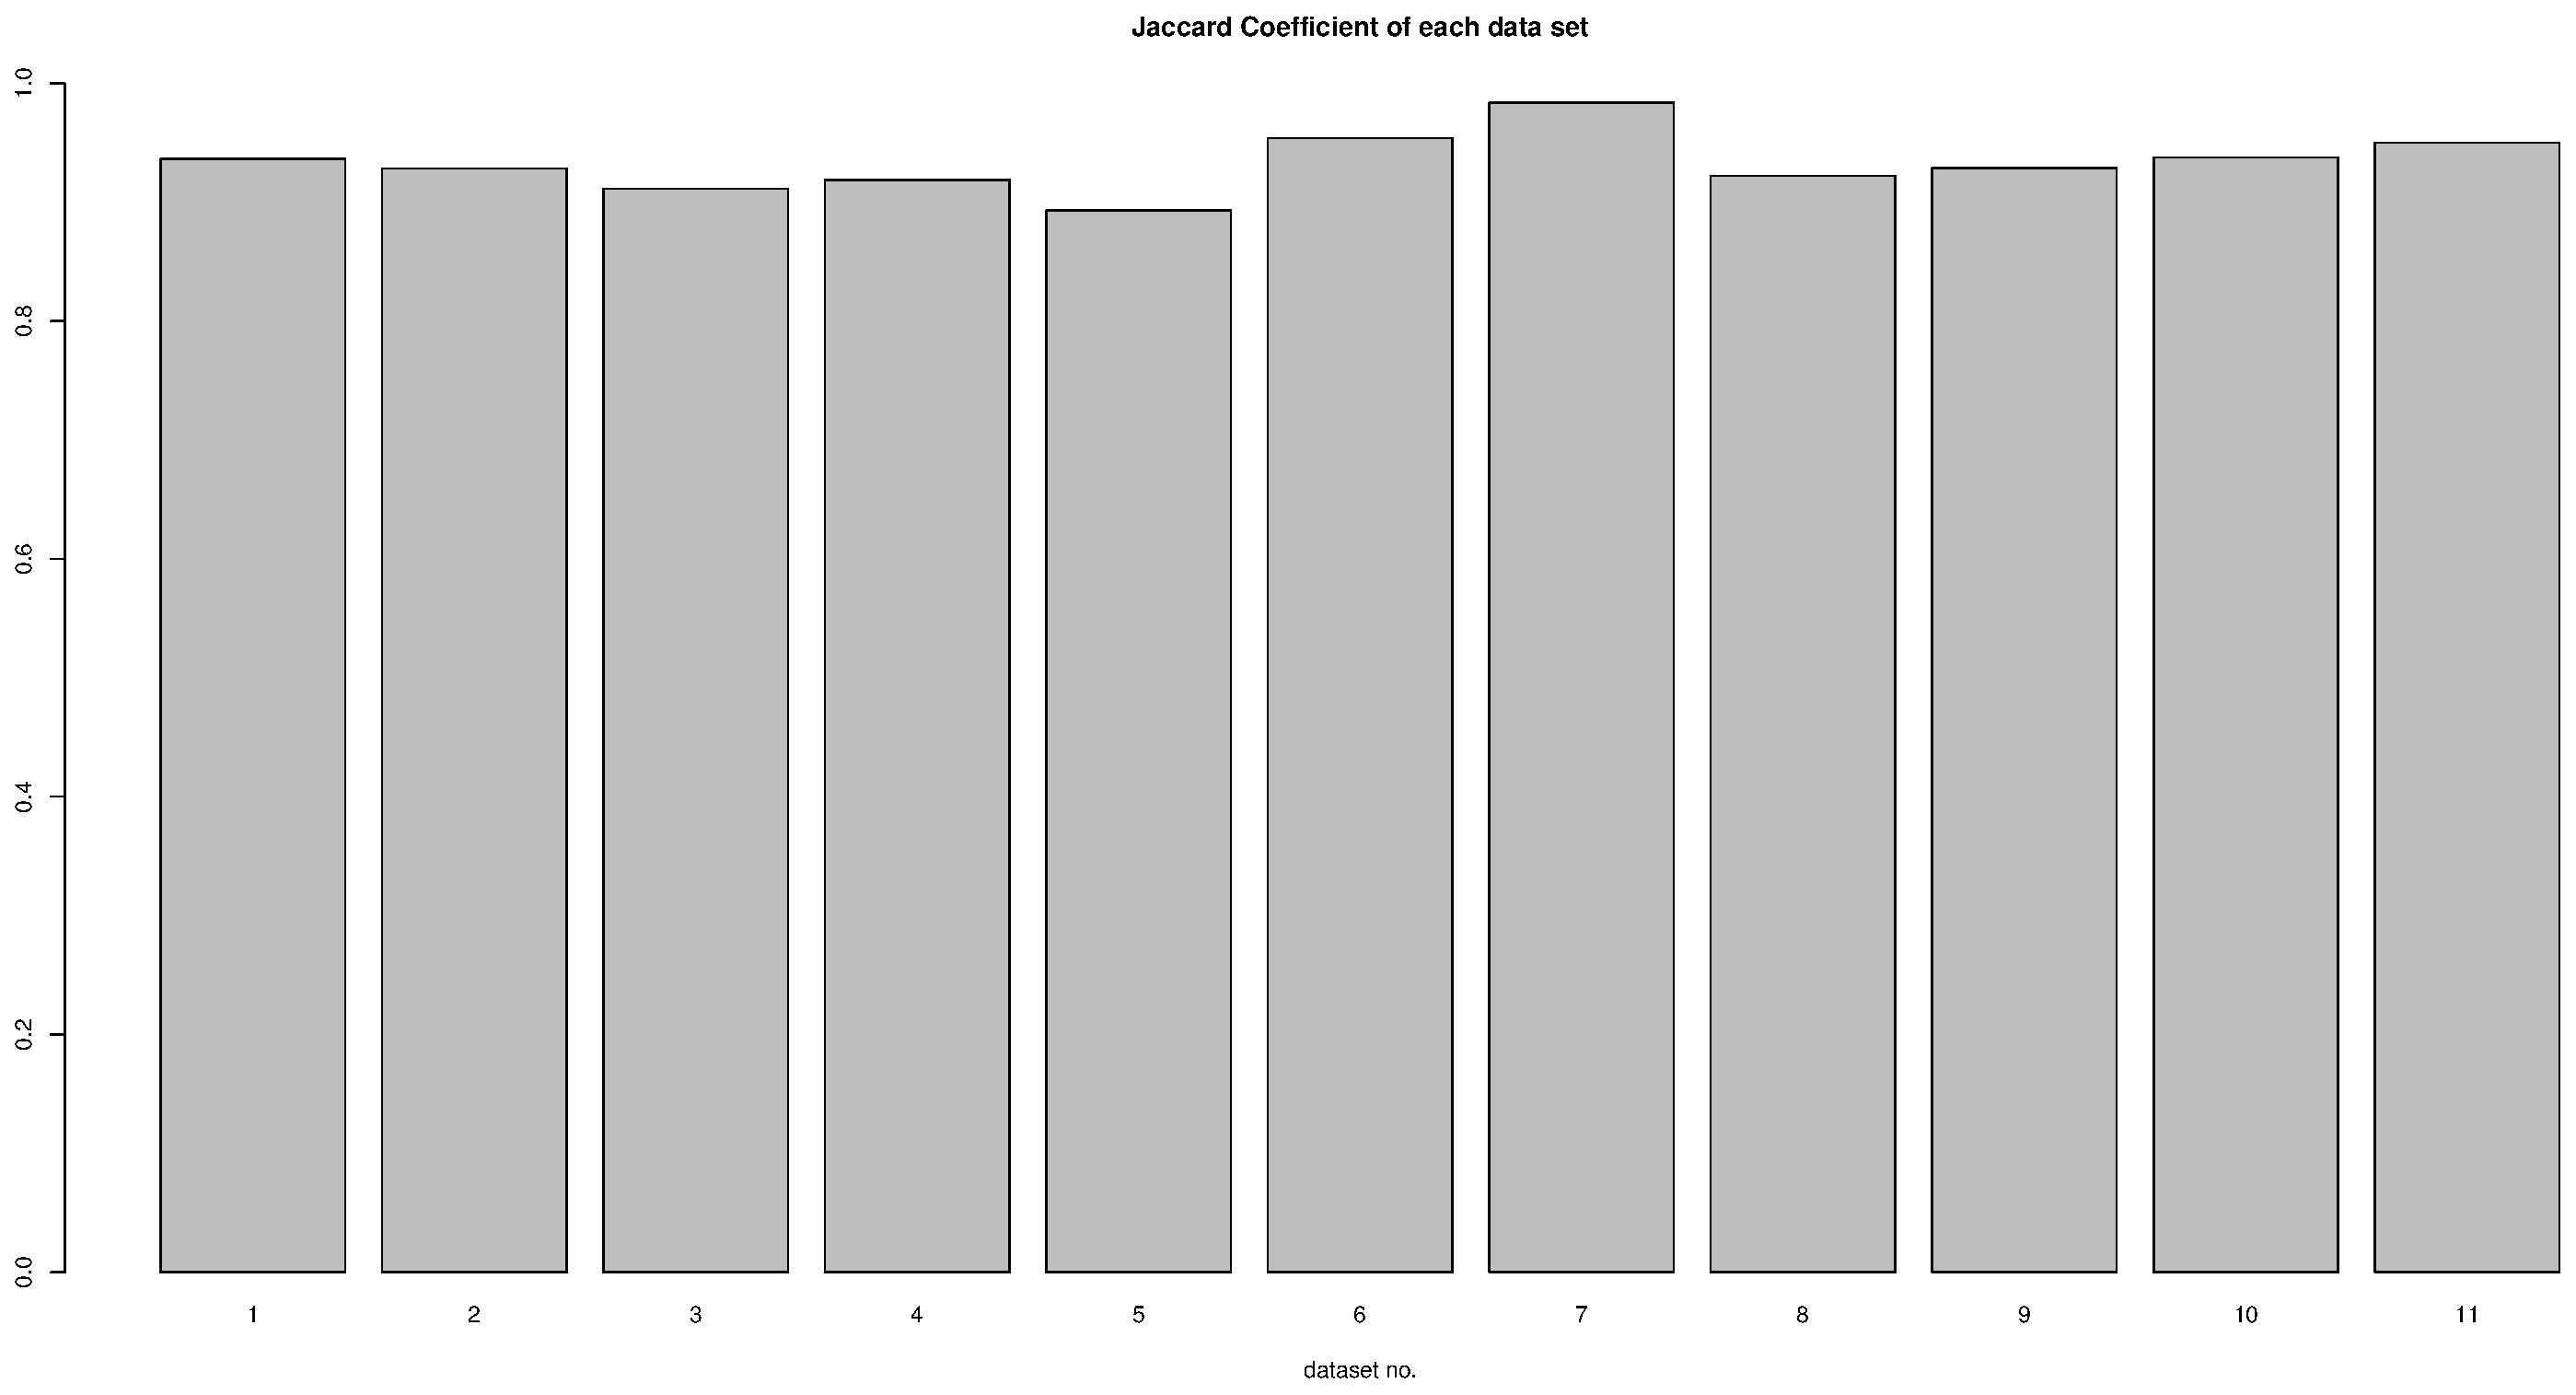
\includegraphics[width=1.8in,height=1.3in]{../../Figures/gac/Jaccard.eps}
\end{figure}
\end{column}
\begin{column}{.5\textwidth}
\onslide<3-4> \begin{figure}[t]
\centering
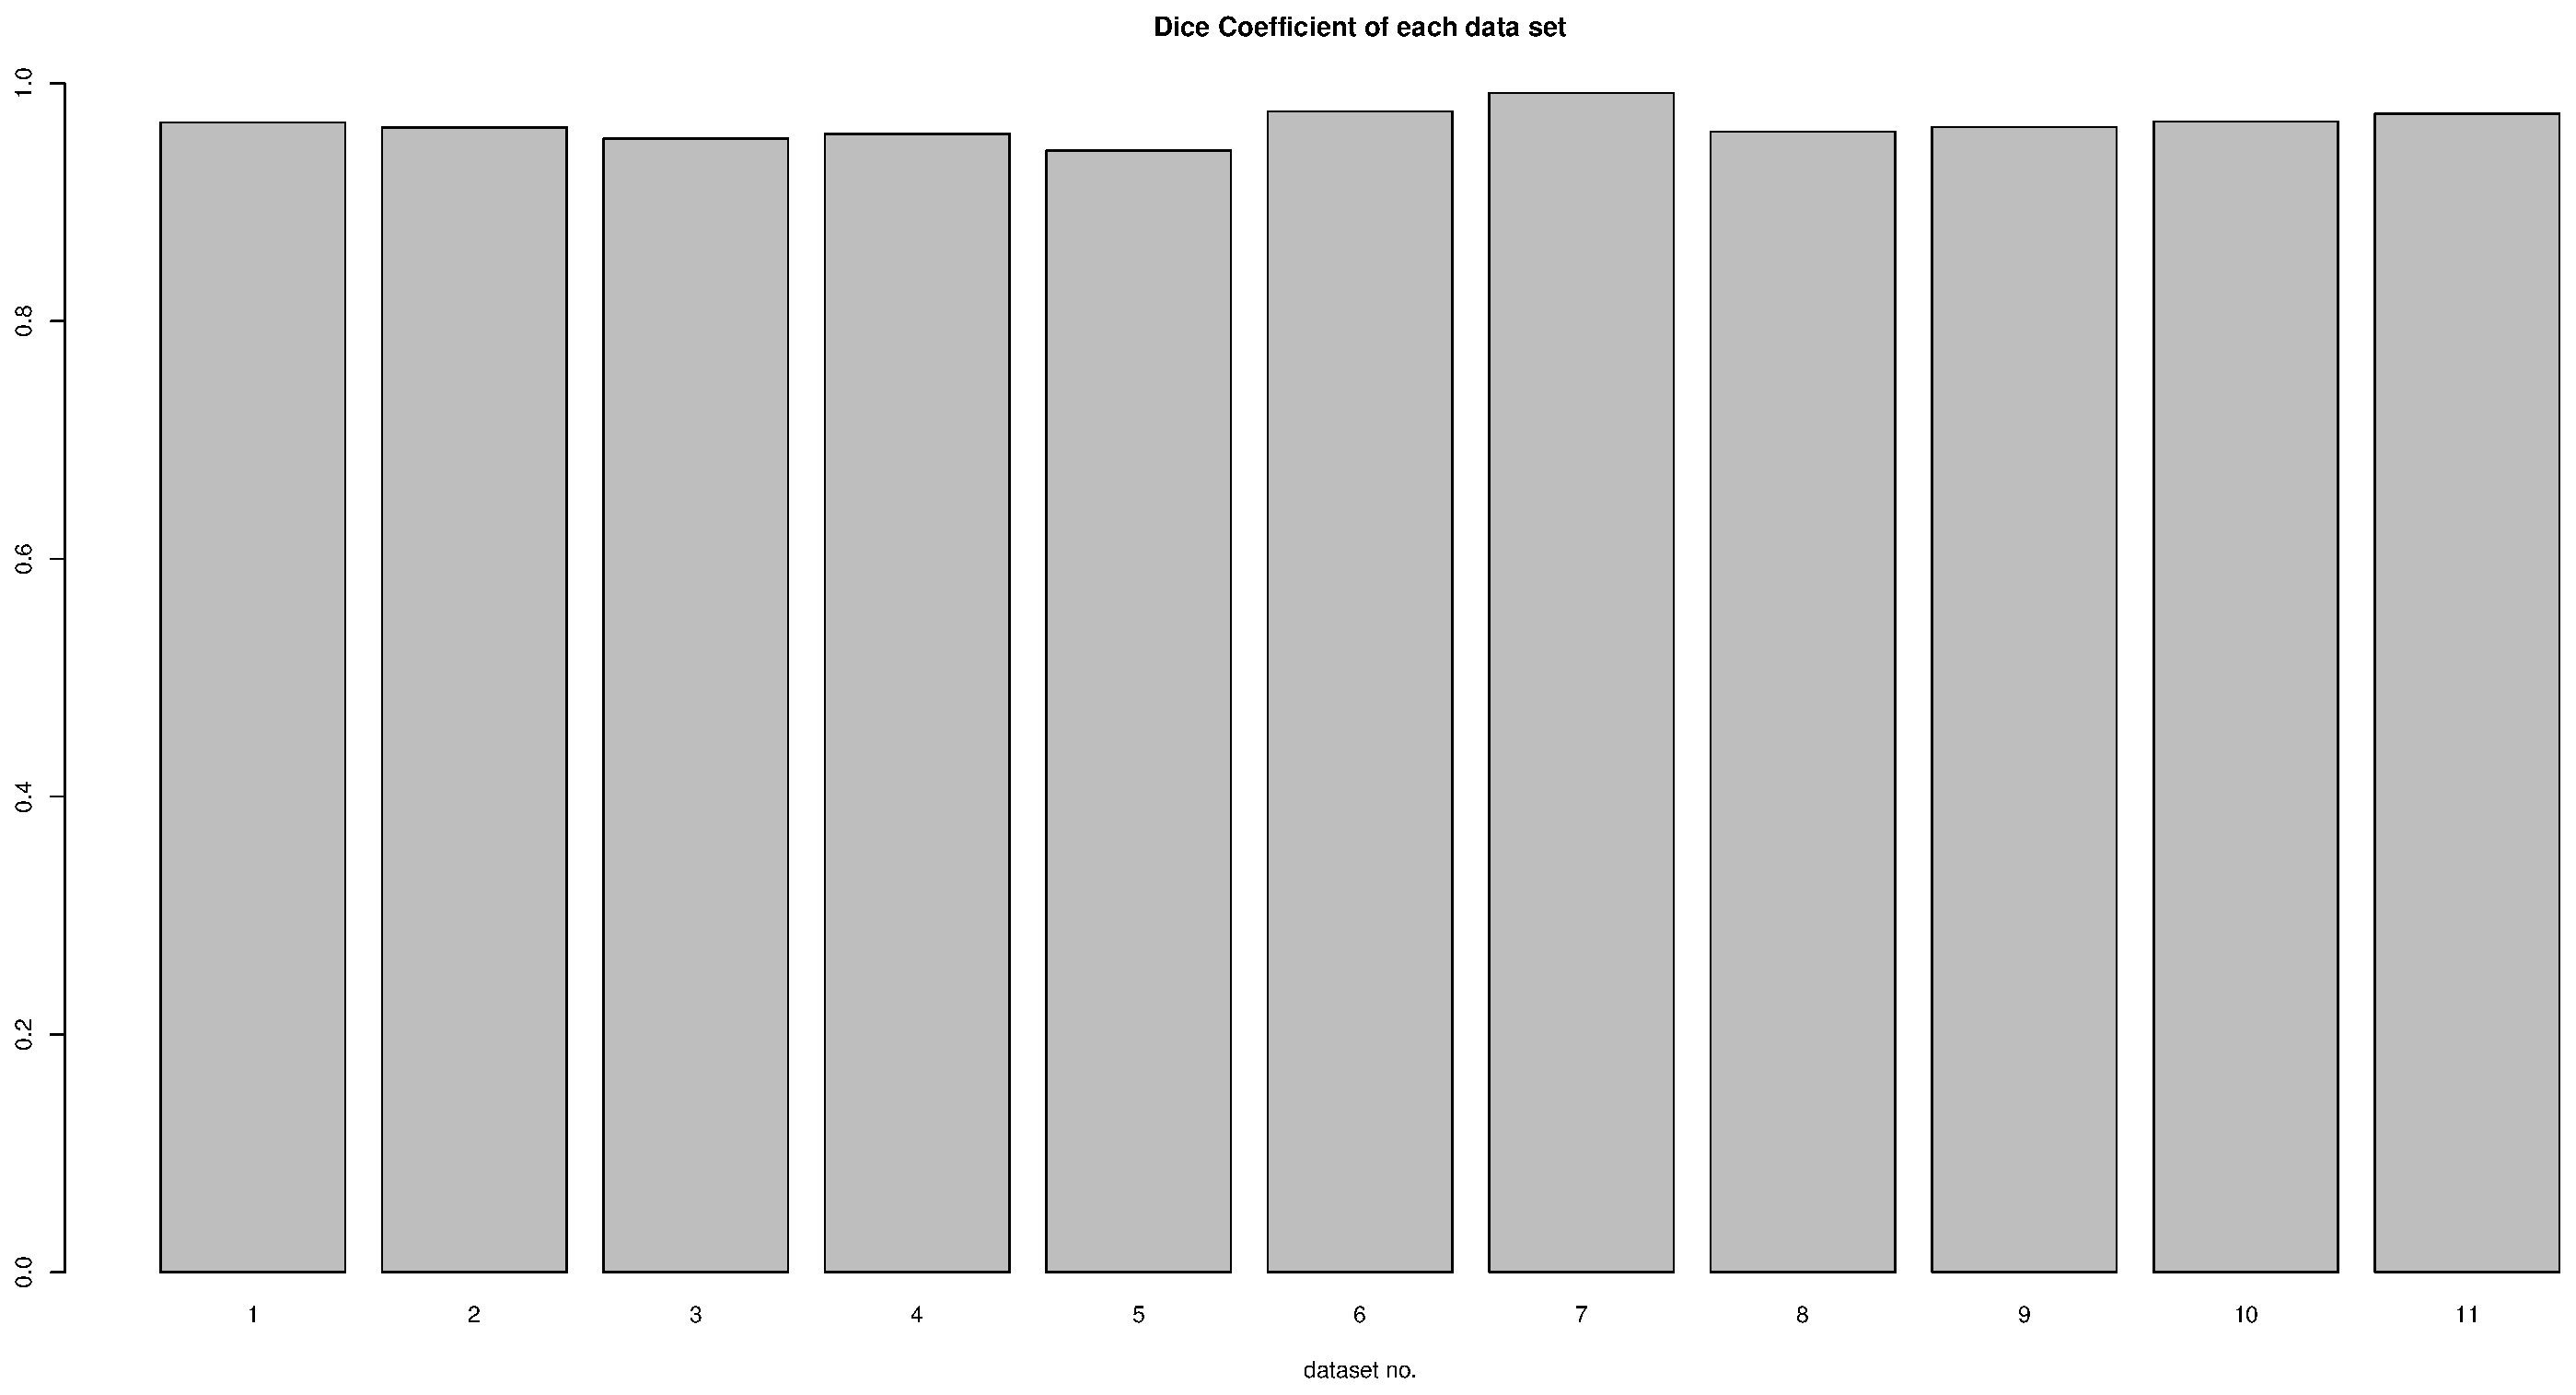
\includegraphics[width=1.8in,height=1.3in]{../../Figures/gac/Dice.eps}
\end{figure}
\end{column}
\end{columns}
\end{frame} 

\begin{frame}
\begin{itemize}
  \item \textbf{主动脉内腔三维模型}:
\end{itemize}
\begin{figure}[t]
\centering
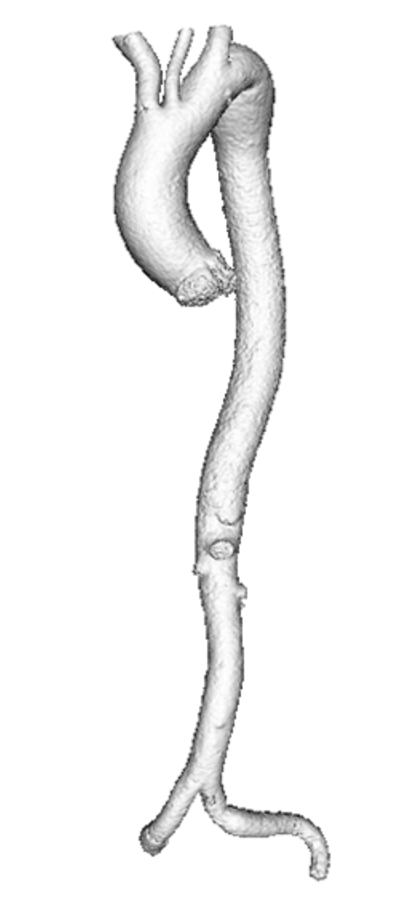
\includegraphics[height=1.8in]{../../Figures/gac/model.eps}
% \caption[主动脉内腔三维模型]{主动脉内腔三维模型。}
% \label{fig:aorta_visualization}
\end{figure} 
\end{frame} 

%# -*- coding:utf-8 -*-
\subsection[心脏分割]{基于测地活动轮廓的心脏近似区域分割}

\begin{frame}
\begin{itemize}
\item \textbf{血管介入仿真中心脏表面模型的作用}
\begin{itemize}
\item 增强虚拟解剖环境的视觉效果
\item 为辨认冠状动脉模型的不同分支提供空间参照物
\end{itemize}
\pause \item \textbf{血管介入仿真中心脏表面模型的获取}
\begin{itemize}
\item 几何形状近似的椭球或者不规则的几何体
\item 未考虑心脏表面模型
\item 医学影像处理方法
\end{itemize}
\pause \item \textbf{心脏近似区域的分割与可视化}
\begin{itemize}
\item 是医学影像领域中的一项极具挑战性的工作
\item 形态特征:不规则的空间形体,可近似看作椭球
\item 分割时的主要困难:搏动致心脏边缘模糊不清,且帧间变化大
\begin{itemize}
\item 只分割心脏的近似区域,得到近似模型,满足仿真需要
\end{itemize}
\end{itemize}
\end{itemize}
\end{frame}

\begin{frame}
\begin{itemize}
  \item \textbf{心脏区域分割流程}:
\end{itemize}
\begin{figure}[t]
\centering
%# -*- coding:utf-8 -*-
\begin{tikzpicture}[scale=.37]

\draw [black,thick,rounded corners] (-3,0) rectangle (3,2);            % binary threshold
\draw [black,thick,rounded corners] (-3,3) rectangle (3,5);  % CURVES

\draw [black,thick,rounded corners] (-8,7) rectangle (-2,9);   % initial contours

\draw [black,thick,rounded corners] (2,7) rectangle (8,9);     % feature images

\draw [black,thick,rounded corners] (-3,11) rectangle (3,13);  % thresholding
\draw [black,thick,rounded corners] (-3,14) rectangle (3,16);  % curvature anisotropic diffusion
\draw [black,thick,rounded corners] (-3,17) rectangle (3,19);  % raw input

\node [above right] at (-2.25,0.25) {\scriptsize \fs \bf 二值阈值滤波};
\node [above right] at (-2.25,3.25) {\scriptsize \fs \bf 测地活动轮廓};

\node [above right] at (-7.65,7.35) {\scriptsize \fs \bf 初始水平集演进};

\node [above right] at (2.82,7.35) {\scriptsize \fs \bf 特征图像计算};

\node [above right] at (-2.3,11.35) {\scriptsize \fs \bf 二值阈值滤波};
\node [above right] at (-2.9,14.35) {\scriptsize \fs \bf 曲率各向异性扩散};
\node [above right] at (-1.95,17.35) {\scriptsize \fs \bf ROI体数据};

\draw [<-,thick] (0,2) -- (0,3);

\draw [<-,thick] (0,5) -- (0,6);
\draw [thick] (-5,6) -- (5,6);
\draw [thick] (-5,6) -- (-5,7);
\draw [thick] (5,6) -- (5,7);

\draw [<-,thick] (-5,9) -- (-5,10);
\draw [<-,thick] (5,9) -- (5,10);
\draw [thick] (-5,10) -- (5,10);
\draw [thick] (0,10) -- (0,11);

\draw [<-,thick] (0,13) -- (0,14);
\draw [<-,thick] (0,16) -- (0,17);

\end{tikzpicture} 
% \includegraphics[height=2.0in]{figures/heart/DataFlow.eps}
% \caption[心脏区域分割流程]{心脏区域分割流程。}
% \label{fig:heart_data_flow}
\end{figure}
\end{frame}

% \begin{frame}
% \begin{itemize}
  % \item \textbf{心脏区域前面观}:
% \end{itemize}
% \begin{figure}[t]
% \centering
% 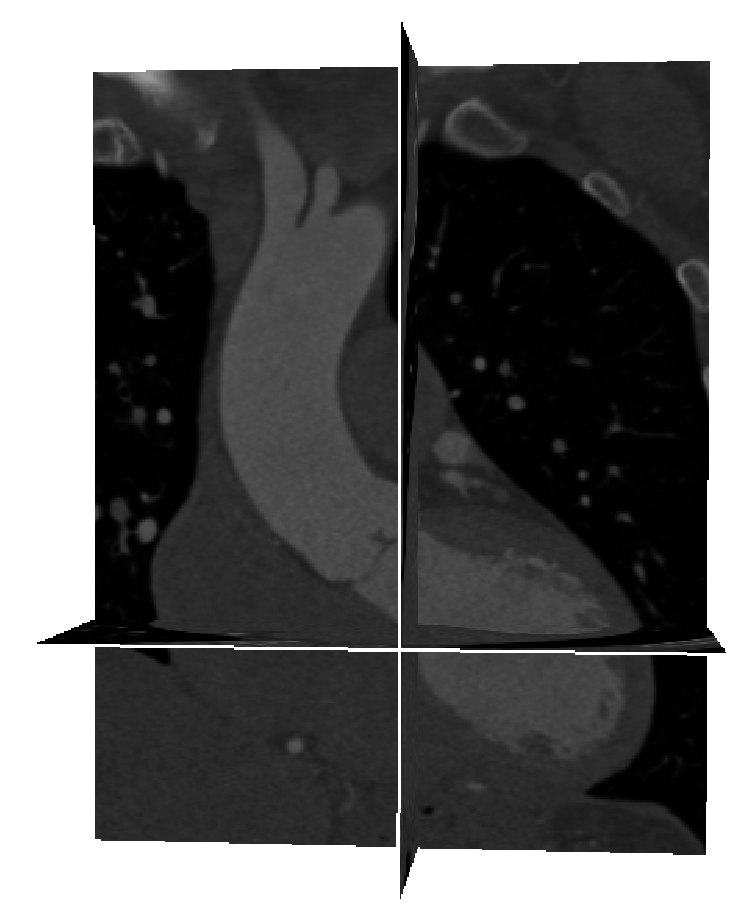
\includegraphics[height=1.5in]{../../Figures/gac/heart/original.eps}
% \end{figure}
% \end{frame}

\begin{frame}
\begin{itemize}
  \item \textbf{二值阈值后心脏区域前面观}:
  \begin{itemize}
    \pause \item 阈值滤波($\text{TH}_{\text{lower}} = 0$,$\text{TH}_{\text{upper}} = 200$)
    \pause \item 注意其中的心脏组织以及大部分血管等都已被除去
  \end{itemize}
\end{itemize}
% \begin{figure}[t]
% \centering
% 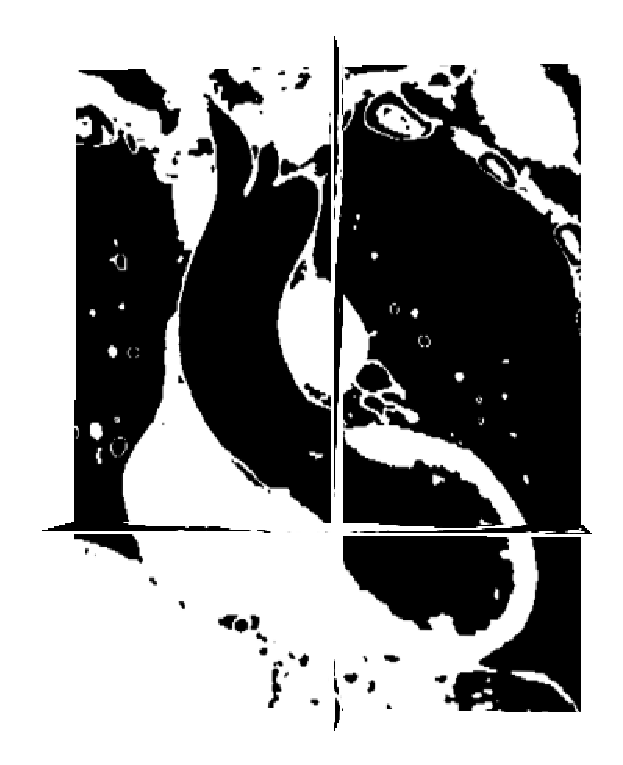
\includegraphics[height=1.5in]{../../Figures/gac/heart/binary_threshold.eps}
% \caption[二值阈值后心脏区域前面观]{二值阈值后心脏区域前面观($\text{TH}_{\text{lower}} = 0$,$\text{TH}_{\text{upper}} = 200$)。注意其中的心包,以及大部分血管等都已被除去。}%
% \label{fig:heart_binary_threshold_experiments}
% \end{figure}
\begin{columns}[b,onlytextwidth]
\begin{column}{.5\textwidth}
\pause \begin{figure}
\centering
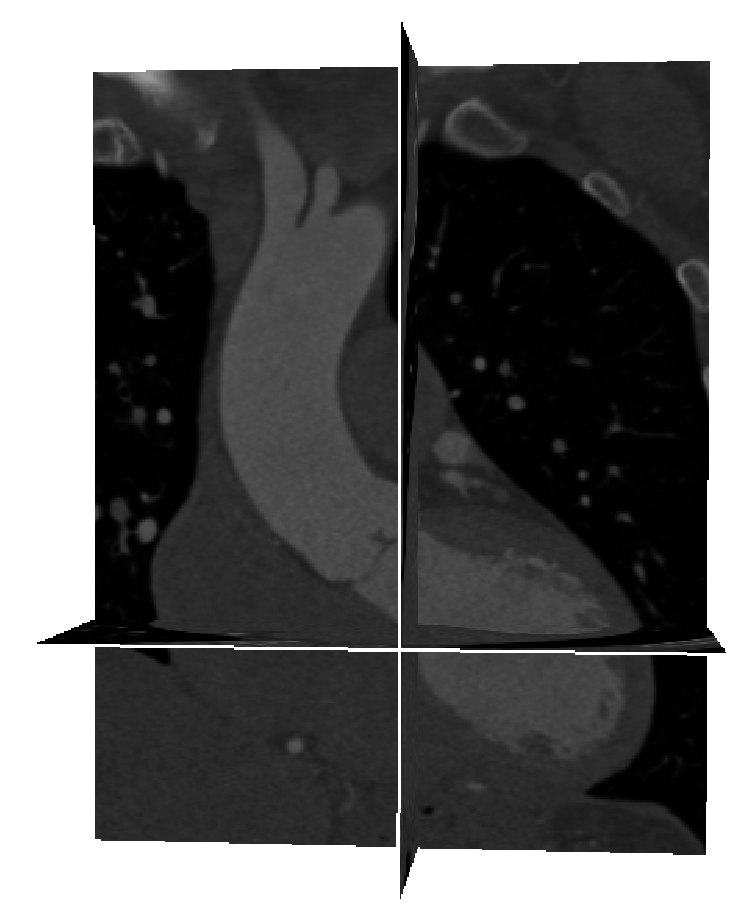
\includegraphics[height=1.5in]{../../Figures/gac/heart/original.eps}
\end{figure}
\end{column}
\begin{column}{.5\textwidth}
\pause \begin{figure}
\centering
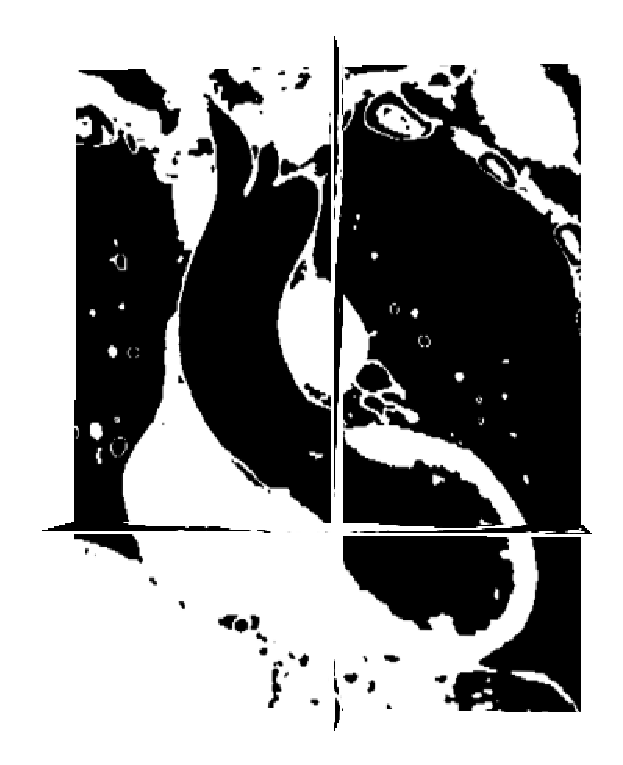
\includegraphics[height=1.5in]{../../Figures/gac/heart/binary_threshold.eps}
\end{figure}
\end{column}
\end{columns}
\end{frame}

\begin{frame}
\begin{itemize}
  \item \textbf{心脏表面模型前面观}:
  % \begin{itemize}
    % \item $\text{TH}_{\text{lower}} = 0$,$\text{TH}_{\text{upper}} = 200$
    % \item 注意其中的心包,以及大部分血管等都已被除去
  % \end{itemize}
\end{itemize}
\begin{figure}[t]
\centering
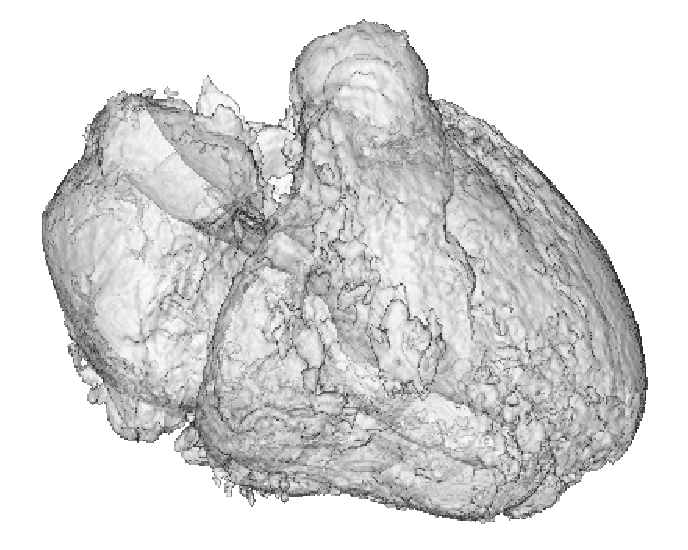
\includegraphics[height=1.5in]{../../Figures/gac/heart/heart.eps}
% \caption[二值阈值后心脏区域前面观]{二值阈值后心脏区域前面观($\text{TH}_{\text{lower}} = 0$,$\text{TH}_{\text{upper}} = 200$)。注意其中的心包,以及大部分血管等都已被除去。}%
% \label{fig:heart_binary_threshold_experiments}
\end{figure}
\end{frame}

\begin{frame}
\begin{itemize}
  \item \textbf{叠加冠状动脉(红色)的心脏模型前面观}:
  % \begin{itemize}
    % \item $\text{TH}_{\text{lower}} = 0$,$\text{TH}_{\text{upper}} = 200$
    % \item 注意其中的心包,以及大部分血管等都已被除去
  % \end{itemize}
\end{itemize}
\begin{figure}[t]
\centering
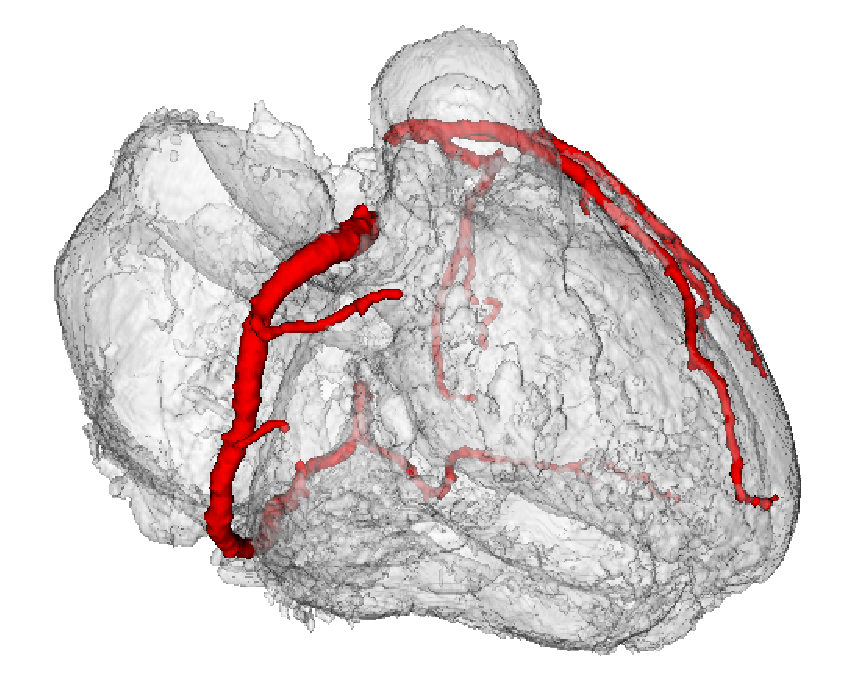
\includegraphics[height=1.5in]{../../Figures/gac/heart/heart_with_ca.eps}
% \caption[二值阈值后心脏区域前面观]{二值阈值后心脏区域前面观($\text{TH}_{\text{lower}} = 0$,$\text{TH}_{\text{upper}} = 200$)。注意其中的心包,以及大部分血管等都已被除去。}%
% \label{fig:heart_binary_threshold_experiments}
\end{figure}
\end{frame} 

% \begin{frame}

% \end{frame} 
 
%# -*- coding:utf-8 -*-
\subsection[冠状动脉分割I]{基于CURVES的冠状动脉分割}

\begin{frame}
\begin{itemize}
\item \textbf{血管介入仿真中冠脉表面模型的作用}
\begin{itemize}
\item 虚拟解剖环境的核心组成部分
\item 血管介入术中病灶所在
\item 虚拟导管交互的硬约束
\end{itemize}
\pause \item \textbf{血管介入仿真中心脏表面模型的获取}
\begin{itemize}
\item 几何形状近似的细管
\item 扫描高精度物理模具
\item 医学影像处理方法
\end{itemize}
\pause \item \textbf{心脏近似区域的分割与可视化}
\begin{itemize}
\item 是医学影像领域中的一项极具挑战性的工作
\item 形态特征:不规则的空间管状物,走向和半径变化复杂
\item 分割时的主要困难:亮度过低不易观察,细节丢失严重
% \begin{itemize}
% \item 只分割心脏的近似区域,得到近似模型,满足仿真需要
% \end{itemize}
\end{itemize}
\end{itemize}
\end{frame}

\begin{frame}
\begin{itemize}
\item \textbf{CURVES方法~[Lorigo(2001)]}
\begin{itemize}
\item 是GAC的一项扩展,仍属水平集方法
\item 计算准则考虑了目标边缘的平滑性
\item 专门用于探测医学体数据中细微复杂的空间线形结构
\item 将线形结构的边界抽象为空间流形
\end{itemize}
\pause \item \textbf{CURVES方法的使用}
\begin{itemize}
\item 需要设置计算的起始点
\item 起始点的设置要考虑到冠状动脉的走向
\end{itemize}
\end{itemize}
\end{frame}

\begin{frame}
\begin{itemize}
\item \textbf{CURVES模型}:使如下的能量泛函最小化
\begin{equation*}
% \label{eqn:coronary_CURVES}
E(\mathcal C) = \oint_0^1 g\left( \left| \nabla I \left( \mathcal{C} \left(  s \right) \right) \right| \right) \left| \mathcal{C}'\left( s \right) \right| ds,
\end{equation*}
\begin{itemize}
\item $E(\cdot)$:能量泛函
\item $\mathcal{C}(\cdot)$:参数化空间曲线
\item $I(\cdot)$:含有待探测目标的图像
\item $g(\cdot)$:一个严格递减函数,且$g > 0$
\end{itemize}
\end{itemize}
\end{frame}

\begin{frame}
\begin{itemize}
\item \textbf{演进方程}:Euler-Lagrange方程,最速下降法求解
\begin{equation*}
\mathcal{C}_t = \frac{\partial \mathcal{C}}{\partial t} = k \mathcal{N} - \frac{g'}{g} \varPi \left( \mathcal{H} \frac{\nabla I}{\left| \nabla I \right|} \right)
\end{equation*}
\begin{itemize}
\item $\varPi(\cdot)$:$\mathcal{C}$在其法平面上的投影
\item $\mathcal{H}(\cdot)$:像素亮度函数的Hessian阵
\item $\frac{g'}{g} \left( \mathcal{H} \frac{\nabla I}{\left| \nabla I \right|} \right)$:辅助向量场
\end{itemize}
\end{itemize}
\end{frame}

\begin{frame}
\begin{itemize}
\item \textbf{更新方程}:嵌入水平集空间
\begin{equation*}
v_t = \frac{\partial v}{\partial t} = \lambda \left( \nabla v, \nabla^2 v \right) + \frac{g'}{g} \nabla v \cdot \mathcal{H} \frac{\nabla I}{ \left| \nabla I \right| }
\end{equation*}
\begin{itemize}
\item $v(\cdot): \mathrm{R}^3 \rightarrow [0, \infty)$:辅助函数,$\mathcal{C}$的零水平集
\item $\lambda \left( \nabla v, \nabla^2 v \right)$:$P_{\nabla v} \nabla^{2} v P_{\nabla v}$较小的特征值
\item $P_{\nabla v} = I - \frac{\nabla v \nabla v^{T}}{\left| \nabla v \right|^{2}}$:在$\nabla v$法平面上的投影, $I$是像素亮度阵
\end{itemize}
\end{itemize}
\end{frame}

\begin{frame}
\begin{itemize}
  \item \textbf{心脏区域的ROI提取}:
  \begin{itemize}
  \pause \item 设定矩形区域的起点和尺寸
  \pause \item 缩小处理区域,减轻运算负担
  \end{itemize}
\end{itemize}
\begin{figure}[t]
\centering
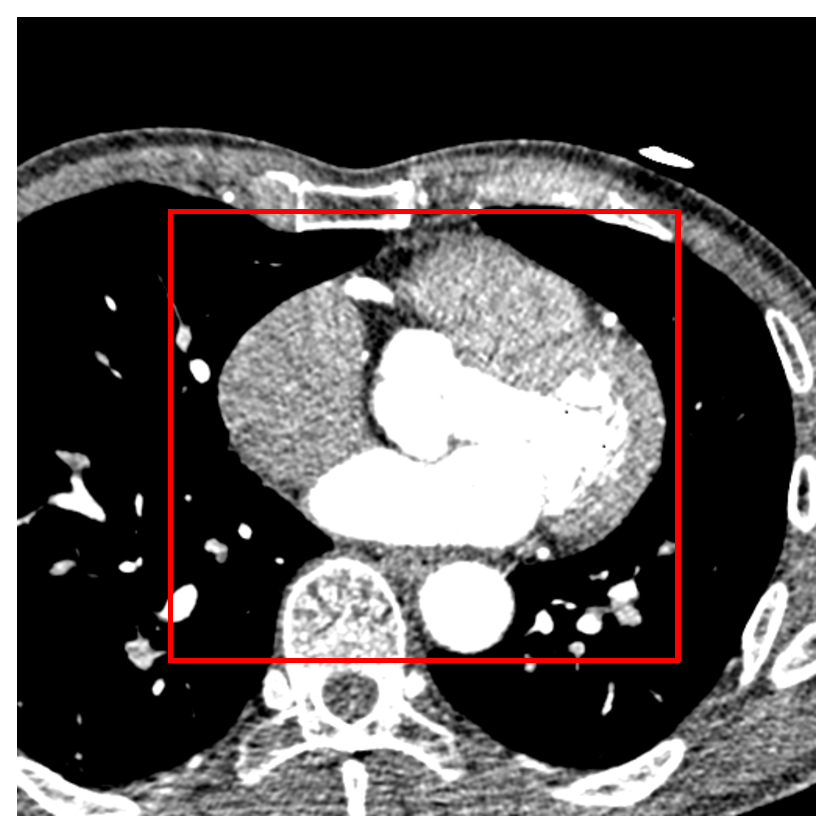
\includegraphics[width=1.5in]{../../Figures/coronary/ROI_Extraction}
% \caption[心脏区域的ROI提取]{心脏区域的ROI提取。}
% \label{fig:coronary_ROI}
\end{figure}
\end{frame}

\begin{frame}
\begin{itemize}
  \item \textbf{基于CURVES的冠状动脉分割流程}:
\end{itemize}
\begin{figure}[t]
\centering
%# -*- coding:utf-8 -*-
\begin{tikzpicture}[scale=.37]

\draw [black,thick,rounded corners] (-3,0) rectangle (3,2);            % binary threshold
\draw [black,thick,rounded corners] (-3,3) rectangle (3,5);  % CURVES

\draw [black,thick,rounded corners] (-8,7) rectangle (-2,9);   % initial contours

\draw [black,thick,rounded corners] (2,7) rectangle (8,9);     % feature images

\draw [black,thick,rounded corners] (-3,11) rectangle (3,13);  % thresholding
\draw [black,thick,rounded corners] (-3,14) rectangle (3,16);  % curvature anisotropic diffusion
\draw [black,thick,rounded corners] (-3,17) rectangle (3,19);  % raw input

\node [above right] at (-2.25,0.25) {\scriptsize \fs \bf 二值阈值滤波};
\node [above right] at (-2.25,3.25) {\scriptsize \fs \bf 测地活动轮廓};

\node [above right] at (-7.65,7.35) {\scriptsize \fs \bf 初始水平集演进};

\node [above right] at (2.82,7.35) {\scriptsize \fs \bf 特征图像计算};

\node [above right] at (-2.3,11.35) {\scriptsize \fs \bf 二值阈值滤波};
\node [above right] at (-2.9,14.35) {\scriptsize \fs \bf 曲率各向异性扩散};
\node [above right] at (-1.95,17.35) {\scriptsize \fs \bf ROI体数据};

\draw [<-,thick] (0,2) -- (0,3);

\draw [<-,thick] (0,5) -- (0,6);
\draw [thick] (-5,6) -- (5,6);
\draw [thick] (-5,6) -- (-5,7);
\draw [thick] (5,6) -- (5,7);

\draw [<-,thick] (-5,9) -- (-5,10);
\draw [<-,thick] (5,9) -- (5,10);
\draw [thick] (-5,10) -- (5,10);
\draw [thick] (0,10) -- (0,11);

\draw [<-,thick] (0,13) -- (0,14);
\draw [<-,thick] (0,16) -- (0,17);

\end{tikzpicture} 
% \includegraphics[width=3.2in]{Figures/coronary/DataFlow}
% \caption[心脏区域的ROI提取]{心脏区域的ROI提取。}
% \label{fig:coronary_ROI}
\end{figure}
\end{frame}

\begin{frame}
\begin{itemize}
  \item \textbf{预处理结果}:
  \begin{enumerate}
    \onslide<1-2> \item 保护物体边缘的平滑处理($\text{传导参数} = 9.0$)
    \onslide<2> \item 阈值滤波($\text{TH}_{\text{lower}} = 160$, $\text{TH}_{\text{upper}} = 600$)
  \end{enumerate}
\end{itemize}
\begin{columns}[b,onlytextwidth]
\begin{column}{.5\textwidth}
\onslide<1-2> \begin{figure}
\centering
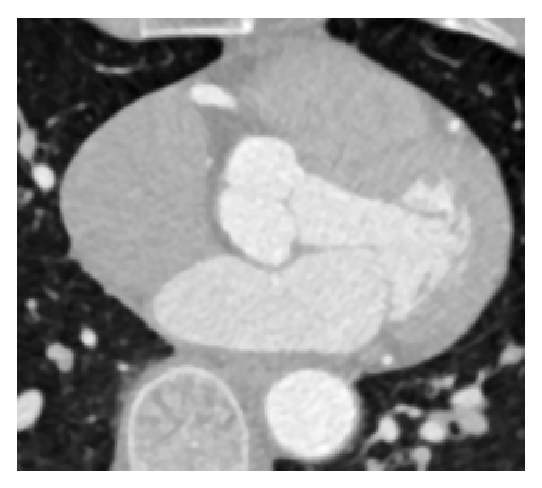
\includegraphics[height=1.5in]{../../Figures/coronary/smooth.eps}
\end{figure}
\end{column}
\begin{column}{.5\textwidth}
\onslide<2> \begin{figure}
\centering
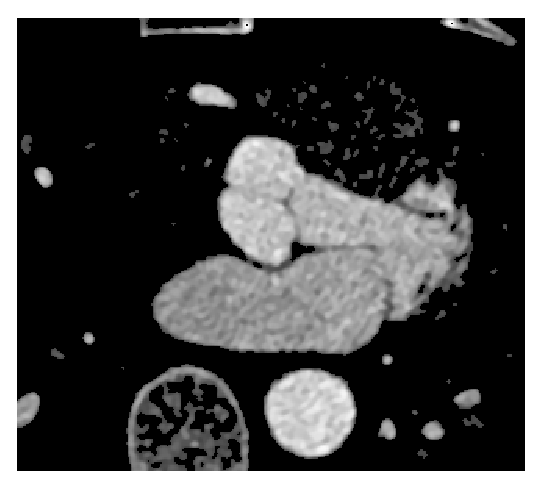
\includegraphics[height=1.5in]{../../Figures/coronary/threshold.eps}
\end{figure}
\end{column}
\end{columns}
\end{frame}

\begin{frame}
\begin{itemize}
  \item \textbf{特征图像计算}:
  \begin{enumerate}
    \onslide<1-2> \item 基于Gaussian核运算所得到的梯度图像($\sigma = 0.9$)
    \onslide<2> \item 通过S函数实现的像素亮度非线性映射($m = -80$, $n = 120$)
  \end{enumerate}
\end{itemize}
\begin{columns}[b,onlytextwidth]
\begin{column}{.5\textwidth}
\onslide<1-2> \begin{figure}
\centering
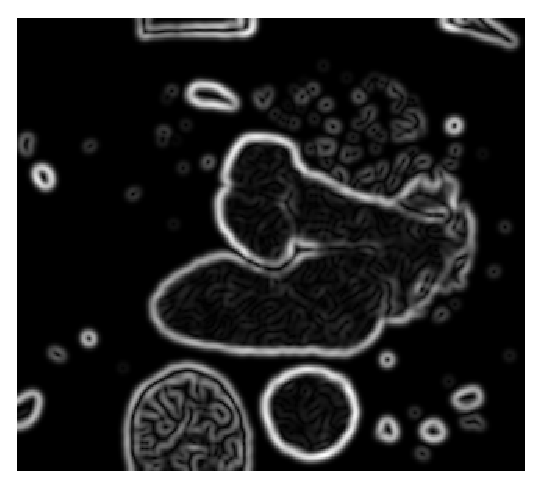
\includegraphics[height=1.5in]{../../Figures/coronary/gradient.eps}
\end{figure}
\end{column}
\begin{column}{.5\textwidth}
\onslide<2> \begin{figure}
\centering
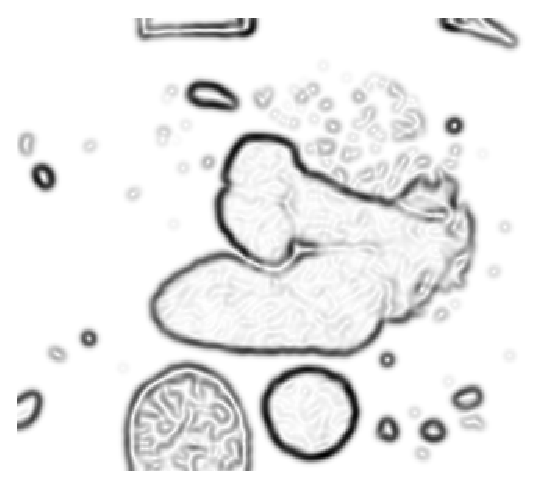
\includegraphics[height=1.5in]{../../Figures/coronary/sigmoid.eps}
\end{figure}
\end{column}
\end{columns}
\end{frame} 

\begin{frame}
\begin{itemize}
  \item \textbf{水平集演进过程}:
  \begin{enumerate}
    \onslide<1-3> \item 通过快速步进算法生成的初始水平集围线
    \onslide<2-3> \item 由CURVES驱动的围线演进结果
    \onslide<3> \item 对演进结果进行二值阈值滤波处理后的结果
  \end{enumerate}
\end{itemize}
\begin{columns}[b,onlytextwidth]
\begin{column}{.3\textwidth}
\onslide<1-3> \begin{figure}
\centering
\setlength{\fboxrule}{0.1pt}
\setlength{\fboxsep}{0cm}
\fbox{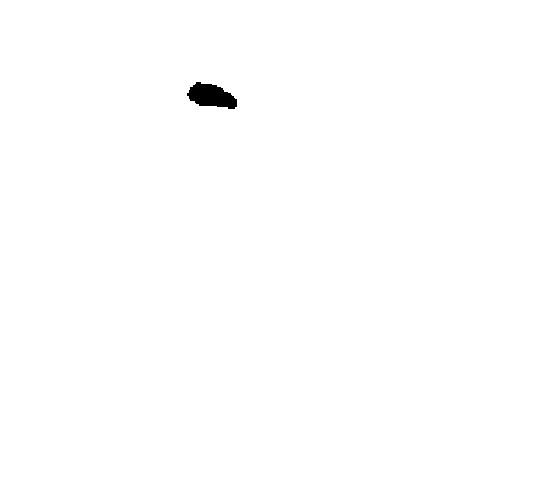
\includegraphics[width=1.2in]{../../Figures/coronary/fastmarching.eps}}
\end{figure}
\end{column}
\begin{column}{.3\textwidth}
\onslide<2-3> \begin{figure}
\centering
\setlength{\fboxrule}{0.1pt}
\setlength{\fboxsep}{0cm}
\fbox{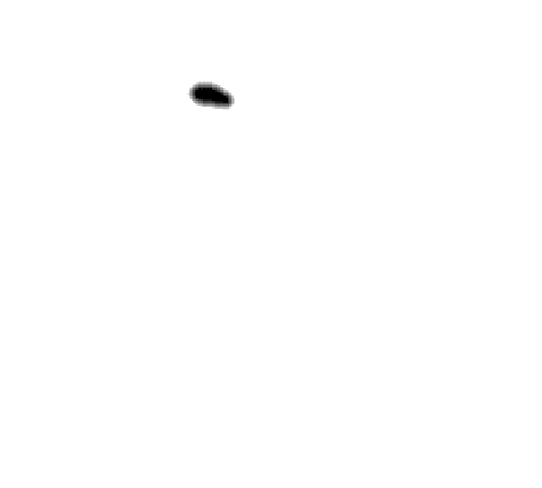
\includegraphics[width=1.2in]{../../Figures/coronary/curves.eps}}
\end{figure}
\end{column}
\begin{column}{.3\textwidth}
\onslide<3> \begin{figure}
\centering
\setlength{\fboxrule}{0.1pt}
\setlength{\fboxsep}{0cm}
\fbox{
\includegraphics[width=1.2in]{../../Figures/coronary/final.eps}}
\end{figure}
\end{column}
\end{columns}
\end{frame} 

\begin{frame}
\begin{itemize}
  \item \textbf{冠状动脉表面模型}:
\end{itemize}
\begin{figure}
\centering
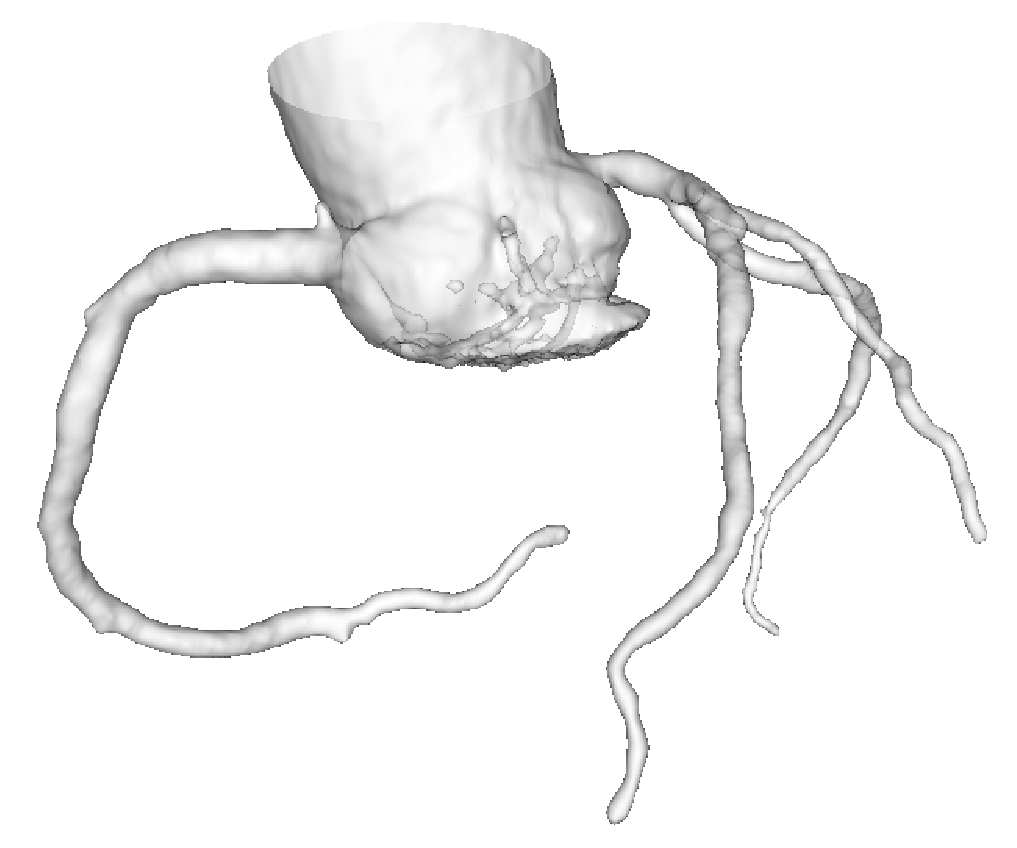
\includegraphics[width=1.5in]{../../Figures/coronary/model}
% \caption[心脏区域的ROI提取]{心脏区域的ROI提取。}
% \label{fig:coronary_ROI}
\end{figure}
\end{frame} 

% \begin{frame}

% \end{frame} 

%# -*- coding:utf-8 -*-
\subsection[冠状动脉分割II]{改进的基于CURVES的冠状动脉分割}

\begin{frame}
\begin{itemize}
\item \textbf{多尺度管状物增强~[Sato(1998)]}
\begin{itemize}
\pause \item \textbf{三维线滤波}:等价为三维图像$I(\cdot)$的Hessian阵的计算:
\begin{gather*}
\mathcal{H} = \nabla^2 I =
\begin{bmatrix}
I_{xx} & I_{xy} & I_{xz} \\ I_{yx} & I_{yy} & I_{yz} \\ I_{zx} & I_{zy} & I_{zz}
\end{bmatrix}
\end{gather*}
\begin{itemize}
\item \textbf{特征值}: $\lambda_1$,$\lambda_2$,和$\lambda_3$,降序排列
\item \textbf{相应的特征向量}: $e_1$,$e_2$,和$e_3$
\end{itemize}
\pause \item \textbf{滤波响应的多尺度整合}:求各尺度响应的最大值
\end{itemize}
\end{itemize}
\end{frame}

\begin{frame}
\begin{itemize}
\item \textbf{增强不同形状所需的特征值}
\end{itemize}
\begin{table}[h]
\renewcommand{\arraystretch}{0.5}
\centering
\begin{tabular*}{80mm}{cc}
\toprule
\hspace{5mm} \bfseries \small{物体形状}  & \hspace{15mm}                    \bfseries \small{特征值}                       \\
\midrule
\hspace{5mm} \small{明亮的管状}          & \hspace{15mm}  \small{$\lambda_1 \approx 0, \lambda_2 \approx \lambda_3 \ll 0$} \\
\hspace{5mm} \small{暗淡的管状}          & \hspace{15mm}  \small{$\lambda_1 \approx 0, \lambda_2 \approx \lambda_3 \gg 0$} \\
\hspace{5mm} \small{明亮的盘状}          & \hspace{15mm}  \small{$\lambda_1 \approx \lambda_2 \approx 0, \lambda_3 \ll 0$} \\
\hspace{5mm} \small{暗淡的盘状}          & \hspace{15mm}  \small{$\lambda_1 \approx \lambda_2 \approx 0, \lambda_3 \gg 0$} \\
\hspace{5mm} \small{明亮的球状}          & \hspace{15mm}  \small{$\lambda_1 \approx \lambda_2 \approx \lambda_3 \ll 0$}    \\
\hspace{5mm} \small{暗淡的球状}          & \hspace{15mm}  \small{$\lambda_1 \approx \lambda_2 \approx \lambda_3 \gg 0$}    \\
\bottomrule
\end{tabular*}
\end{table}
\end{frame}

\begin{frame}
\begin{itemize}
\item \textbf{线形测度} (\alert{$\lambda_1 \approx 0$ and $\lambda_2 \approx \lambda_3 \ll 0$})
\pause \begin{equation*}
\lambda_{123} =
\begin{cases}
\left| \lambda_3 \right| \left( \frac{\lambda_2}{\lambda_3} \right)^{\gamma_{23}} \left( 1 + \frac{\lambda_1}{\left| \lambda_2 \right|} \right)^{\gamma_{12}},        & \lambda_1 \le 0 \\%
\left| \lambda_3 \right| \left( \frac{\lambda_2}{\lambda_3} \right)^{\gamma_{23}} \left( 1 - \alpha \frac{\lambda_1}{\left| \lambda_2 \right|} \right)^{\gamma_{12}}, & \frac{\left| \lambda_2 \right|}{\alpha} > \lambda_1 > 0 \\%
0,                                                                                                                                                                    & \text{其它} %
\end{cases}
\end{equation*}
% \end{itemize}
\begin{itemize}
\pause \item \textbf{附加参数}:$\gamma_{12}$,$\gamma_{23}$,和$\alpha$,全部为正
\begin{itemize}
\item $\gamma_{12} \in [0, \infty)$:辨别出分支结构与噪音以及伪分支结构
\item $\gamma_{23} \in [0, \infty)$:控制图像锐度
\item $\alpha \in (0, 1.0]$:对于任意$\lambda_1$,保持函数最后一项的对称性
\end{itemize}
\end{itemize}
\end{itemize}
\end{frame}

\begin{frame}
\begin{itemize}
  \item \textbf{心脏区域的VOI提取}:
  \begin{itemize}
  \pause \item 设定长方体区域的起点和尺寸
  \pause \item 缩小处理区域,减轻运算负担
  \end{itemize}
\end{itemize}
\begin{figure}[t]
\centering
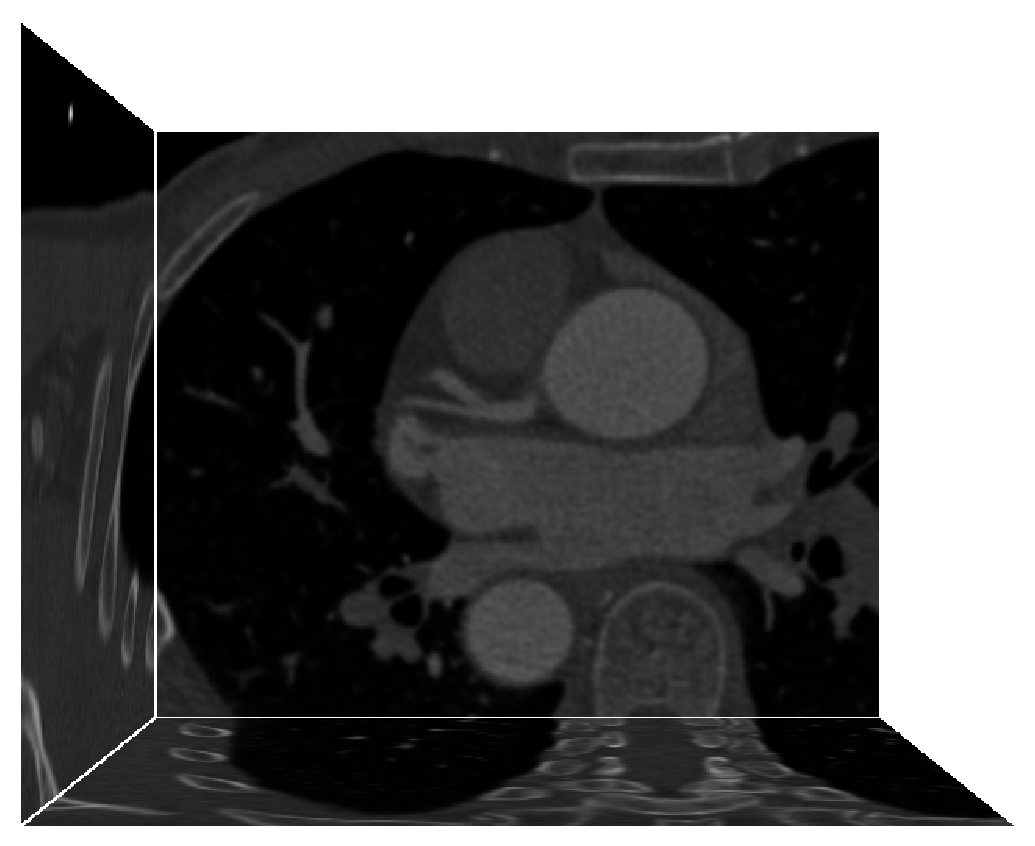
\includegraphics[width=1.5in]{../../Figures/coronary/coronary_enhanced/original}
% \caption[心脏区域的ROI提取]{心脏区域的ROI提取。}
% \label{fig:coronary_ROI}
\end{figure}
\end{frame}

\begin{frame}
\begin{itemize}
  \item \textbf{改进的冠状动脉分割流程}:
\end{itemize}
\begin{figure}[t]
\centering
%# -*- coding:utf-8 -*-
\begin{tikzpicture}[scale=.37]

\draw [black,thick,rounded corners] (-3,0) rectangle (3,2);            % binary threshold
\draw [black,thick,rounded corners] (-3,3) rectangle (3,5);  % CURVES

\draw [black,thick,rounded corners] (-8,7) rectangle (-2,9);   % initial contours

\draw [black,thick,rounded corners] (2,7) rectangle (8,9);     % feature images

\draw [black,thick,rounded corners] (-3,11) rectangle (3,13);  % thresholding
\draw [black,thick,rounded corners] (-3,14) rectangle (3,16);  % curvature anisotropic diffusion
\draw [black,thick,rounded corners] (-3,17) rectangle (3,19);  % raw input

\node [above right] at (-2.25,0.25) {\scriptsize \fs \bf 二值阈值滤波};
\node [above right] at (-2.25,3.25) {\scriptsize \fs \bf 测地活动轮廓};

\node [above right] at (-7.65,7.35) {\scriptsize \fs \bf 初始水平集演进};

\node [above right] at (2.82,7.35) {\scriptsize \fs \bf 特征图像计算};

\node [above right] at (-2.3,11.35) {\scriptsize \fs \bf 二值阈值滤波};
\node [above right] at (-2.9,14.35) {\scriptsize \fs \bf 曲率各向异性扩散};
\node [above right] at (-1.95,17.35) {\scriptsize \fs \bf ROI体数据};

\draw [<-,thick] (0,2) -- (0,3);

\draw [<-,thick] (0,5) -- (0,6);
\draw [thick] (-5,6) -- (5,6);
\draw [thick] (-5,6) -- (-5,7);
\draw [thick] (5,6) -- (5,7);

\draw [<-,thick] (-5,9) -- (-5,10);
\draw [<-,thick] (5,9) -- (5,10);
\draw [thick] (-5,10) -- (5,10);
\draw [thick] (0,10) -- (0,11);

\draw [<-,thick] (0,13) -- (0,14);
\draw [<-,thick] (0,16) -- (0,17);

\end{tikzpicture} 
% \includegraphics[width=3.2in]{Figures/coronary/DataFlow}
% \caption[心脏区域的ROI提取]{心脏区域的ROI提取。}
% \label{fig:coronary_ROI}
\end{figure}
\end{frame}

\begin{frame}
\begin{itemize}
  \item \textbf{基于vesselness的预处理}:
  \begin{enumerate}
    \onslide<1-3> \item 二值阈值滤波($\text{TH}_{\text{lower}} = 300$, $\text{TH}_{\text{upper}} = 600$)
    \onslide<3> \item 管状物体增强($\sigma = 0.9$, $\gamma_{12} = 0.1$, $\gamma_{23} = 2.0$)
  \end{enumerate}
\end{itemize}
\begin{columns}[b,onlytextwidth]
\begin{column}{.5\textwidth}
\onslide<2-3> \begin{figure}[t]
\centering
\includegraphics[height=1.5in]{../../Figures/coronary/coronary_enhanced/binary1.eps}
\end{figure}
\end{column}
\begin{column}{.5\textwidth}
\onslide<3> \begin{figure}[t]
\centering
\includegraphics[height=1.5in]{../../Figures/coronary/coronary_enhanced/hessian.eps}
\end{figure}
\end{column}
\end{columns}
% \centering{\textbf{\alert 增强后的管状物亮度值过低,且不均匀}}
\end{frame}

\begin{frame}
\begin{itemize}
  \item \textbf{两种像素亮度处理结果对比}:
  \begin{enumerate}
    \onslide<1-3> \item 非线性亮度映射($m = 80$, $n = 120$)
    \onslide<3> \item 二值阈值滤波($\text{TH}_{\text{lower}} = 40$, $\text{TH}_{\text{upper}} = 200$)
  \end{enumerate}
\end{itemize}
\begin{columns}[b,onlytextwidth]
\begin{column}{.5\textwidth}
\onslide<2-3> \begin{figure}[t]
\centering
\includegraphics[height=1.5in]{../../Figures/coronary/coronary_enhanced/sigmoid.eps}
\end{figure}
\end{column}
\begin{column}{.5\textwidth}
\onslide<3> \begin{figure}[t]
\centering
\includegraphics[height=1.5in]{../../Figures/coronary/coronary_enhanced/binary2.eps}
\end{figure}
\end{column}
\end{columns}
\end{frame}

\begin{frame}
\begin{itemize}
  \item \textbf{增强处理后的CURVES演进}:
\end{itemize}
\begin{figure}[t]
\centering
\includegraphics[width=1.5in]{../../Figures/coronary/coronary_enhanced/curves}
% \caption[心脏区域的ROI提取]{心脏区域的ROI提取。}
% \label{fig:coronary_ROI}
\end{figure}
\end{frame}

\begin{frame}
\begin{itemize}
  \item \textbf{冠状动脉模型对比}:
  \begin{enumerate}
    \onslide<1-3> \item 传统CURVES演进
    \onslide<3> \item 管状物增强后的CURVES演进
  \end{enumerate}
\end{itemize}
\begin{columns}[b,onlytextwidth]
\begin{column}{.5\textwidth}
\onslide<2-3> \begin{figure}[t]
\centering
\includegraphics[height=1.2in]{../../Figures/coronary/coronary_enhanced/model_conventional.eps}
\end{figure}
\end{column}
\begin{column}{.5\textwidth}
\onslide<3> \begin{figure}[t]
\centering
\includegraphics[height=1.2in]{../../Figures/coronary/coronary_enhanced/model_enhanced.eps}
\end{figure}
\end{column}
\end{columns}
\end{frame}

% \begin{frame}

% \end{frame}

% \begin{frame}

% \end{frame} 
\section{医学可视化}
%# -*- coding:utf-8 -*-
\subsection[模型数据优化]{面向交互仿真的血管系统模型数据优化}

\begin{frame}
\begin{itemize}
\item \textbf{血管介入仿真中血管表面模型的要求}
\begin{itemize}
\pause \item 提供虚拟解剖环境的可视化
\begin{itemize}
\item 外观平整,圆滑,无破损,无层叠
\end{itemize}
\pause \item 满足与虚拟导管的交互仿真需求
\begin{itemize}
\item 数据量:多边形面片数量(多边形的顶点)
\end{itemize}
\end{itemize}
\pause \item \textbf{血管介入仿真中血管表面模型的优化处理}
\begin{itemize}
\pause \item 顶点连接性检验
\pause \item 无损的表面平整和修补
\pause \item 多边形精简(基于“平均表面”准则)
\end{itemize}
% \item \textbf{心脏近似区域的分割与可视化}
% \begin{itemize}
% \item 是医学影像领域中的一项极具挑战性的工作
% \item 形态特征:不规则的空间管状物,走向和半径变化复杂
% \item 分割时的主要困难:亮度过低不易观察,细节丢失严重
% \begin{itemize}
% \item 只分割心脏的近似区域,得到近似模型,满足仿真需要
% \end{itemize}
% \end{itemize}
\end{itemize}
\end{frame}

% \begin{frame}
% \begin{itemize}
  % \item \textbf{血管表面模型优化流程}:
% \end{itemize}
% \begin{figure}[t]
% \centering
% %# -*- coding:utf-8 -*-
\begin{tikzpicture}[scale=.37]

\draw [black,thick,rounded corners] (-3,0) rectangle (3,2);            % binary threshold
\draw [black,thick,rounded corners] (-3,3) rectangle (3,5);  % CURVES

\draw [black,thick,rounded corners] (-8,7) rectangle (-2,9);   % initial contours

\draw [black,thick,rounded corners] (2,7) rectangle (8,9);     % feature images

\draw [black,thick,rounded corners] (-3,11) rectangle (3,13);  % thresholding
\draw [black,thick,rounded corners] (-3,14) rectangle (3,16);  % curvature anisotropic diffusion
\draw [black,thick,rounded corners] (-3,17) rectangle (3,19);  % raw input

\node [above right] at (-2.25,0.25) {\scriptsize \fs \bf 二值阈值滤波};
\node [above right] at (-2.25,3.25) {\scriptsize \fs \bf 测地活动轮廓};

\node [above right] at (-7.65,7.35) {\scriptsize \fs \bf 初始水平集演进};

\node [above right] at (2.82,7.35) {\scriptsize \fs \bf 特征图像计算};

\node [above right] at (-2.3,11.35) {\scriptsize \fs \bf 二值阈值滤波};
\node [above right] at (-2.9,14.35) {\scriptsize \fs \bf 曲率各向异性扩散};
\node [above right] at (-1.95,17.35) {\scriptsize \fs \bf ROI体数据};

\draw [<-,thick] (0,2) -- (0,3);

\draw [<-,thick] (0,5) -- (0,6);
\draw [thick] (-5,6) -- (5,6);
\draw [thick] (-5,6) -- (-5,7);
\draw [thick] (5,6) -- (5,7);

\draw [<-,thick] (-5,9) -- (-5,10);
\draw [<-,thick] (5,9) -- (5,10);
\draw [thick] (-5,10) -- (5,10);
\draw [thick] (0,10) -- (0,11);

\draw [<-,thick] (0,13) -- (0,14);
\draw [<-,thick] (0,16) -- (0,17);

\end{tikzpicture} 
% \end{figure}
% \end{frame}

\begin{frame}
\begin{itemize}
  \item \textbf{表面中顶点位置的五种情形~[Schroeder(1992)]}
  \begin{itemize}
    \onslide<1-5> \item 简单情形
    \onslide<2-5> \item 复杂情形
    \onslide<3-5> \item 边缘情形
    \onslide<4-5> \item 边缘内部情形
    \onslide<5> \item 拐角情形
  \end{itemize}
\end{itemize}
\begin{figure}
\begin{minipage}[t]{0.8\linewidth}
\centering
% top
\subfigure{
\onslide<1-5> 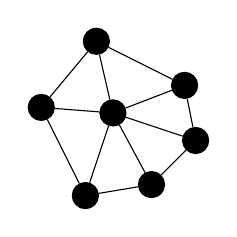
\begin{tikzpicture}[scale=.7,every node/.style={draw,shape=circle,fill=black,minimum size=1pt}]
% vertices
\path (0.5,1.5) node (p0) {}
(0,0) node (p1) {}
(1.2,0.2) node (p2) {}
(2,1) node (p3) {}
(1.8,2) node (p4) {}
(0.2,2.8) node (p5) {}
(-0.8,1.6) node (p6) {};
% edges
\draw (p0) -- (p1)
(p0) -- (p2)
(p0) -- (p3)
(p0) -- (p4)
(p0) -- (p5)
(p0) -- (p6)
(p1) -- (p2)
(p2) -- (p3)
(p3) -- (p4)
(p4) -- (p5)
(p5) -- (p6)
(p6) -- (p1);
\end{tikzpicture}
\quad
\onslide<2-5> 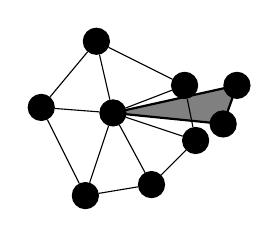
\begin{tikzpicture}[scale=.7,every node/.style={draw,shape=circle,fill=black,minimum size=1pt}]
\draw [fill=gray,thick] (0.5,1.5) -- (2.5,1.3) -- (2.75,2) -- (0.5,1.5);
% vertices
\path (0.5,1.5) node (p0) {}
(0,0) node (p1) {}
(1.2,0.2) node (p2) {}
(2,1) node (p3) {}
(1.8,2) node (p4) {}
(0.2,2.8) node (p5) {}
(-0.8,1.6) node (p6) {}
(2.5,1.3) node (p7) {}
(2.75,2) node (p8) {};
% edges
\draw (p0) -- (p1)
(p0) -- (p2)
(p0) -- (p3)
(p0) -- (p4)
(p0) -- (p5)
(p0) -- (p6)
(p1) -- (p2)
(p2) -- (p3)
(p3) -- (p4)
(p4) -- (p5)
(p5) -- (p6)
(p6) -- (p1);
\end{tikzpicture}
\quad
\onslide<3-5> 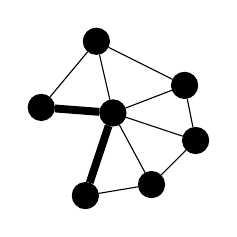
\begin{tikzpicture}[scale=.7,every node/.style={draw,shape=circle,fill=black,minimum size=1pt}]
% vertices
\path (0.5,1.5) node (p0) {}
(0,0) node (p1) {}
(1.2,0.2) node (p2) {}
(2,1) node (p3) {}
(1.8,2) node (p4) {}
(0.2,2.8) node (p5) {}
(-0.8,1.6) node (p6) {};
% edges
\draw (p0) -- (p1)
(p0) -- (p2)
(p0) -- (p3)
(p0) -- (p4)
(p0) -- (p5)
(p0) -- (p6)
(p1) -- (p2)
(p2) -- (p3)
(p3) -- (p4)
(p4) -- (p5)
(p5) -- (p6);
\draw [line width=.1cm] (p1) -- (p0) -- (p6);
\end{tikzpicture}
}
% bottom
\subfigure{
\onslide<4-5> 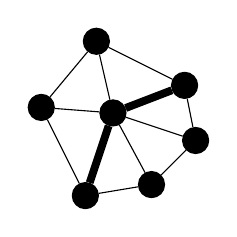
\begin{tikzpicture}[scale=.7,every node/.style={draw,shape=circle,fill=black,minimum size=1pt}]
% vertices
\path (0.5,1.5) node (p0) {}
(0,0) node (p1) {}
(1.2,0.2) node (p2) {}
(2,1) node (p3) {}
(1.8,2) node (p4) {}
(0.2,2.8) node (p5) {}
(-0.8,1.6) node (p6) {};
% edges
\draw (p0) -- (p1)
(p0) -- (p2)
(p0) -- (p3)
(p0) -- (p4)
(p0) -- (p5)
(p0) -- (p6)
(p1) -- (p2)
(p2) -- (p3)
(p3) -- (p4)
(p4) -- (p5)
(p5) -- (p6)
(p6) -- (p1);
\draw [line width=.1cm] (p1) -- (p0) -- (p4);
\end{tikzpicture}
\quad
\onslide<5> 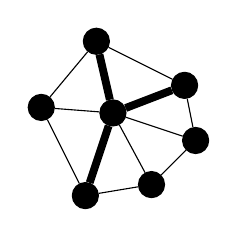
\begin{tikzpicture}[scale=.7,every node/.style={draw,shape=circle,fill=black,minimum size=1pt}]
% vertices
\path (0.5,1.5) node (p0) {}
(0,0) node (p1) {}
(1.2,0.2) node (p2) {}
(2,1) node (p3) {}
(1.8,2) node (p4) {}
(0.2,2.8) node (p5) {}
(-0.8,1.6) node (p6) {};
% edges
\draw (p0) -- (p1)
(p0) -- (p2)
(p0) -- (p3)
(p0) -- (p4)
(p0) -- (p5)
(p0) -- (p6)
(p1) -- (p2)
(p2) -- (p3)
(p3) -- (p4)
(p4) -- (p5)
(p5) -- (p6)
(p6) -- (p1);
\draw [line width=.1cm] (p1) -- (p0) -- (p4);
\draw [line width=.1cm] (p0) -- (p5);
\end{tikzpicture}
}	
\end{minipage}
\end{figure}
\end{frame}

\begin{frame}
\begin{itemize}
  \item \textbf{削减顶点引起的多边形减少~[Schroeder(1992)]}
  \begin{itemize}
    \onslide<1-2> \item 简单情形:削减前的多边形数量:$6$,削减后的多边形数量:$4$
    \onslide<2> \item 边缘情形:削减前的多边形数量:$5$,削减后的多边形数量:$4$
  \end{itemize}
\end{itemize}
\begin{figure}
\begin{minipage}[t]{0.8\linewidth}
\centering
% top
\subfigure{
\onslide<1-2> 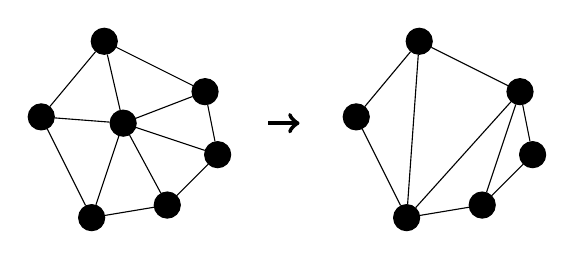
\begin{tikzpicture}[scale=.8,every node/.style={draw,shape=circle,fill=black,minimum size=3pt}]
% vertices
\path (0.5,1.5) node (p0) {}
(0,0) node (p1) {}
(1.2,0.2) node (p2) {}
(2,1) node (p3) {}
(1.8,2) node (p4) {}
(0.2,2.8) node (p5) {}
(-0.8,1.6) node (p6) {};
\path %(5.5,1.5) node (p7) {}
(5,0) node (p8) {}
(6.2,0.2) node (p9) {}
(7,1) node (p10) {}
(6.8,2) node (p11) {}
(5.2,2.8) node (p12) {}
(4.2,1.6) node (p13) {};
% edges
\draw (p0) -- (p1)
(p0) -- (p2)
(p0) -- (p3)
(p0) -- (p4)
(p0) -- (p5)
(p0) -- (p6)
(p1) -- (p2)
(p2) -- (p3)
(p3) -- (p4)
(p4) -- (p5)
(p5) -- (p6)
(p6) -- (p1);
\draw (p8) -- (p9)
(p9) -- (p10)
(p10) -- (p11)
(p11) -- (p12)
(p12) -- (p13)
(p13) -- (p8)
(p8) -- (p12)
(p8) -- (p11)
(p9) -- (p11);
% draw arrow
\draw [->,ultra thick] (2.8,1.5) -- (3.3,1.5);
\end{tikzpicture}
}
% bottom
\subfigure{
\onslide<2> 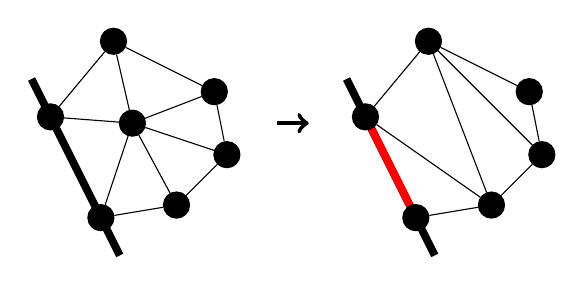
\begin{tikzpicture}[scale=.8,every node/.style={draw,shape=circle,fill=black,minimum size=3pt}]
% vertices
\path (0.5,1.5) node (p0) {}
(0,0) node (p1) {}
(1.2,0.2) node (p2) {}
(2,1) node (p3) {}
(1.8,2) node (p4) {}
(0.2,2.8) node (p5) {}
(-0.8,1.6) node (p6) {};
\path %(5.5,1.5) node (p7) {}
(5,0) node (p8) {}
(6.2,0.2) node (p9) {}
(7,1) node (p10) {}
(6.8,2) node (p11) {}
(5.2,2.8) node (p12) {}
(4.2,1.6) node (p13) {};
% edges
\draw (p0) -- (p1)
(p0) -- (p2)
(p0) -- (p3)
(p0) -- (p4)
(p0) -- (p5)
(p0) -- (p6)
(p1) -- (p2)
(p2) -- (p3)
(p3) -- (p4)
(p4) -- (p5)
(p5) -- (p6);
\draw [line width=0.1cm] (-1.1,2.2) -- (0.3,-0.6);
\draw (p8) -- (p9)
(p9) -- (p10)
(p10) -- (p11)
(p11) -- (p12)
(p12) -- (p13)
(p13) -- (p8)
(p9) -- (p13)
(p9) -- (p12)
(p10) -- (p12);
\draw [line width=0.1cm] (3.9,2.2) -- (5.3,-0.6);
\draw [line width=0.1cm,red] (p8) -- (p13);
% draw arrow
\draw [->,ultra thick] (2.8,1.5) -- (3.3,1.5);
\end{tikzpicture}
}	
\end{minipage}
\end{figure}
\end{frame}

\begin{frame}
\begin{itemize}
  \item \textbf{表面模型的VOI提取及连接性检验}:
\end{itemize}
\begin{figure}[t]
\centering
\includegraphics[height=2.0in]{../../Figures/postprocessing/mesh/original.eps}
\qquad
\raisebox{20mm}{
\centering
\renewcommand{\arraystretch}{0.5}
\begin{tabular*}{40mm}{lc}
\toprule
~                & \small{多边形数量} \\
\midrule
\small{检验前}   & \small{$74,307$}  \\
\small{检验后}   & \small{$74,307$}  \\
\bottomrule
\end{tabular*}
}
\end{figure}
% }
% \caption[表面模型的VOI提取及连接性检验]{表面模型的VOI提取及连接性检验。}
% \label{fig:mesh_connectivity}
\end{frame}

\begin{frame}
\begin{itemize}
  \item \textbf{设置不同参数获得的平滑结果}:($N$:迭代次数;$\delta$:带宽)
  \begin{itemize}
  \item \textbf{目的}:除去噪声,填补漏洞
  \end{itemize}
\end{itemize}
\begin{figure}[t]
\renewcommand{\arraystretch}{0.5}
% \caption[为平滑算法设置不同的参数所获得的结果]{为平滑算法设置不同的参数所获得的结果($N$:迭代次数;$\delta$:带宽)}
% \label{tbl:mesh_smooth}
\centering
\begin{tabular}{|l|c|c|c|}
\hline
\bigstrut ~                                   & \raisebox{-1mm}{$N = 30$}                                     & \raisebox{-1mm}{$N = 60$}                                     & \raisebox{-1mm}{$N = 100$}                                     \\
\hline
\bigstrut[t] \raisebox{0mm}{$\delta = 0.1$}  & \Includegraphics[height=1.0in]{../../Figures/postprocessing/mesh/smooth_30_1.eps}  & \Includegraphics[height=1.0in]{../../Figures/postprocessing/mesh/smooth_60_1.eps}  & \Includegraphics[height=1.0in]{../../Figures/postprocessing/mesh/smooth_100_1.eps}  \\
\hline
\bigstrut[b] \raisebox{0mm}{$\delta = 0.01$} & \Includegraphics[height=1.0in]{../../Figures/postprocessing/mesh/smooth_30_01.eps} & \Includegraphics[height=1.0in]{../../Figures/postprocessing/mesh/smooth_60_01.eps} & \Includegraphics[height=1.0in]{../../Figures/postprocessing/mesh/smooth_100_01.eps} \\
\hline
\end{tabular}
% \caption[设置不同参数获得的平滑结果(优化)]{设置不同参数获得的平滑结果。($N$:迭代次数;$\delta$:带宽)}
% \label{fig:mesh_smooth}
\end{figure}
\end{frame}

\begin{frame}
\begin{itemize}
  \item \textbf{设置不同参数获得的精简}:(精简率公式:$R = \frac{Q_r}{Q}$)
\end{itemize}
\begin{figure}[t]
\begin{table}[t]
\renewcommand{\arraystretch}{0.5}
% \caption[为削减算法设置不同参数所获得的结果]{为平滑算法设置不同的参数所获得的结果($N$:迭代次数;$\delta$:带宽)}
% \label{tbl:mesh_decimate}
\centering
\begin{tabular}{|l|c|c|c|}
\hline
\bigstrut ~                                    & \raisebox{-1mm}{$10\%$}                                                                 & \raisebox{-1mm}{$90\%$}                                                               & \raisebox{-1mm}{$99\%$}                                     \\
\hline
\bigstrut[t] \raisebox{0mm}{\small{表面模型}} & \Includegraphics[height=1.0in]{../../Figures/postprocessing/mesh/smooth_100_01_d10.eps}     & \Includegraphics[height=1.0in]{../../Figures/postprocessing/mesh/smooth_100_01_d90.eps}   & \Includegraphics[height=1.0in]{../../Figures/postprocessing/mesh/smooth_100_01_d99.eps}   \\
\hline
\bigstrut[b] \raisebox{0mm}{\small{线框模型}} & \Includegraphics[height=1.0in]{../../Figures/postprocessing/mesh/smooth_100_01_d10_w.eps}   & \Includegraphics[height=1.0in]{../../Figures/postprocessing/mesh/smooth_100_01_d90_w.eps} & \Includegraphics[height=1.0in]{../../Figures/postprocessing/mesh/smooth_100_01_d99_w.eps} \\
\hline
\end{tabular}
% \caption[设置不同参数获得的精简]{设置不同参数获得的精简:上排展示了削减率分别为$10\%$,$90\%$,$99\%$时的结果;下排展示了上排相应削减结果所对应的线框表示。}
% \label{fig:mesh_decimate}
\end{table}
\end{figure}
\end{frame}

\begin{frame}
\begin{itemize}
  \item \textbf{削减率与削减后的多边形数量}:
\end{itemize}
\begin{table}[h]
\renewcommand{\arraystretch}{0.5}
% \caption[削减率与削减后的多边形数量]{削减率与削减后的多边形数量}
% \label{tbl:mesh_decimate}
\centering
\begin{tabular*}{90mm}{c r r r r r}
\toprule
% \bfseries      & \bfseries Quantity of polygonal surfaces \\
\hspace{2mm} \small{削减率 ($\%$)}  &     \small{$10$} &     \small{$50$} &     \small{$75$} &    \small{$90$} &  \small{$99$} \\
\midrule
\hspace{2mm} \small{多边形数量}     & \small{$66,875$} & \small{$37,153$} & \small{$18,576$} & \small{$7,430$} & \small{$743$} \\
\bottomrule
\end{tabular*}
\end{table}
\end{frame}

\begin{frame}
\begin{itemize}
\item \textbf{交互仿真的指标} (fps $=$ frames per second)
\begin{itemize}
\item \textbf{初始fps}:当虚拟导管进入血管模型时的fps值
\item \textbf{平均fps}:模型中心线上五个给定位置处fps的平均值
\item \textbf{成功}: 将虚拟导管推送至血管模型内部某个预设位置
\end{itemize}
\end{itemize}
\end{frame}

\begin{frame}
\begin{itemize}
  \item \textbf{精简率与fps——情形I}:本章实验模型
\end{itemize}
\begin{table}[t]
\renewcommand{\arraystretch}{0.5}
% \caption[精简率与fps——情形I]{精简率与fps——情形I}
% \label{tbl:mesh_FPS1}
\centering
\begin{tabular*}{90mm}{c r r r r r}
\toprule
\hspace{5mm} \small{精简率($\%$)}           & \small{$10$} & \small{$50$} & \small{$75$} & \small{$90$} & \small{$99$} \\
\midrule
\hspace{5mm} \small{仿真初始fps}              & \small{$30$} & \small{$35$} & \small{$38$} & \small{$41$} & \small{$42$} \\
\midrule
\hspace{5mm} \small{仿真平均fps}              &  \small{$6$} & \small{$10$} & \small{$15$} & \small{$18$} & \small{$30$} \\
\midrule
\hspace{5mm} \small{是否完成仿真?(是/否)}  &  \small{否}  &  \small{否}  & \small{是}   & \small{是}   & \small{是}   \\
\bottomrule
\end{tabular*}
\end{table}
\end{frame}

\begin{frame}
\begin{itemize}
  \item \textbf{精简率与fps——情形II}:完整血管模型
\end{itemize}
\begin{table}[t]
\renewcommand{\arraystretch}{0.5}
% \caption[精简率与fps——情形II]{精简率与fps——情形II}
% \label{tbl:mesh_FPS2}
\centering
\begin{tabular*}{80mm}{c r r r r r}
\toprule
\hspace{5mm} \small{精简率($\%$)}           & \small{$90$} & \small{$95$} & \small{$99$} \\
\midrule
\hspace{5mm} \small{仿真初始fps}              & \small{$20$} & \small{$32$} & \small{$31$} \\
\midrule
\hspace{5mm} \small{仿真平均fps}              &  \small{$4$} &  \small{$6$} & \small{$11$} \\
\midrule
\hspace{5mm} \small{是否完成仿真?(是/否)}  &  \small{否}  &  \small{否}  & \small{是}   \\
\bottomrule
\end{tabular*}
\end{table}
\end{frame}

% \begin{frame}

% \end{frame} 
%# -*- coding:utf-8 -*-
\subsection[中心线提取]{基于Voronoi图的血管模型中心线提取}

\begin{frame}
\begin{itemize}
\item \textbf{血管介入仿真中血管模型中心线的作用}
\begin{itemize}
\pause \item 提供虚拟解剖环境中的血管的几何信息
\begin{itemize}
\item 走向,半径,分岔位置
\end{itemize}
\pause \item 为虚拟导管行进状态的探测提供基准
\begin{itemize}
\item 状态探测:沿中心线均匀分布的空心球(半径小于血管内径)
\end{itemize}
\end{itemize}
\pause \item \textbf{血管介入仿真中血管模型中心线的提取}
\begin{itemize}
\pause \item 顶点连接性检验
\pause \item 无损的表面平整和修补
\pause \item 表面细分
\pause \item 中心线提取
\end{itemize}
% \item \textbf{心脏近似区域的分割与可视化}
% \begin{itemize}
% \item 是医学影像领域中的一项极具挑战性的工作
% \item 形态特征:不规则的空间管状物,走向和半径变化复杂
% \item 分割时的主要困难:亮度过低不易观察,细节丢失严重
% \begin{itemize}
% \item 只分割心脏的近似区域,得到近似模型,满足仿真需要
% \end{itemize}
% \end{itemize}
\end{itemize}
\end{frame}

% \begin{frame}
% \begin{itemize}
% \item Butterfly scheme vs. Improved butterfly scheme
% \begin{itemize}
% \item Butterfly scheme
% \begin{itemize}
% \item can produce refined surface over regular triangular surface (all vertices have valence 6)
% \item can produce undesirable artifacts at vertices with valence other than 6
% \end{itemize}
% \end{itemize}
% \begin{itemize}
% \item Improved butterfly scheme
% \begin{itemize}
% \item can produce refined surface over both regular and irregular (not all vertices have valence 6) triangular surface
% \end{itemize}
% \end{itemize}
% \end{itemize}
% \end{frame}

\begin{frame}
\begin{itemize}
\item \textbf{中心线(中心轴)} : 
\begin{itemize}
\item 物体的最大内切圆(2D)或最大内切球(3D)形心的轨迹~[Amenta(2001)]
\item 为仿真中的过程建模提供有效形状描述
\end{itemize}
\onslide<1-5> \item 中心线提取的四类方法:
\begin{itemize}
\onslide<2-5> \item 拓扑薄化
\onslide<3-5> \item 距离变换
\onslide<4-5> \item 草原之火("prairie fire")
\onslide<5> \item \alert{Voronoi图(VD)}
\end{itemize}
\end{itemize}
\end{frame}

\begin{frame}
\begin{itemize}
\item \textbf{Voronoi图}:
\begin{itemize}
\item 平面或三维形体中心线的离散化估计
\end{itemize}
\item \textbf{中心线}
\begin{itemize}
\item 模型表面内部VD的最短作用路径~[Antiga(2003)]
\begin{itemize}
% \item \alert{中心点}:到表面边界最短距离局部最大
\item \alert{作用路径}:连接VD上两个顶点的连线
\end{itemize}
\item 中心点通过求取作用路径线积分的最小值获得
\begin{itemize}
\item \alert{中心点}:到表面边界最短距离局部最大
% \item \alert{作用路径}:连接VD上两个顶点的连线
\end{itemize}
\end{itemize}
\end{itemize}
\end{frame}

\begin{frame}
\begin{itemize}
\item 从VD上某给定起始点开始计算Eikonal方程
\begin{equation*}
\left| \nabla T \right| = \frac{1}{R(u)}
\end{equation*}
\begin{itemize}
\item $T$:到达时刻
\item $R$:$T$时刻最大内切球的半径
\item $u$:VD的参数空间
\end{itemize}
\item 中心线则利用最速下降法求得
\begin{equation*}
\frac{d}{ds} c = - \nabla T
\end{equation*}
\begin{itemize}
\item $c$:中心线
\item $s$:$c$的参数空间
\end{itemize}
\end{itemize}
\end{frame}

% \begin{frame}
% \begin{itemize}
  % \item \textbf{表面模型中心线提取流程}:
% \end{itemize}
% \begin{figure}[t]
% \centering
% %# -*- coding:utf-8 -*-
\begin{tikzpicture}[scale=.37]

\draw [black,thick,rounded corners] (-3,0) rectangle (3,2);            % binary threshold
\draw [black,thick,rounded corners] (-3,3) rectangle (3,5);  % CURVES

\draw [black,thick,rounded corners] (-8,7) rectangle (-2,9);   % initial contours

\draw [black,thick,rounded corners] (2,7) rectangle (8,9);     % feature images

\draw [black,thick,rounded corners] (-3,11) rectangle (3,13);  % thresholding
\draw [black,thick,rounded corners] (-3,14) rectangle (3,16);  % curvature anisotropic diffusion
\draw [black,thick,rounded corners] (-3,17) rectangle (3,19);  % raw input

\node [above right] at (-2.25,0.25) {\scriptsize \fs \bf 二值阈值滤波};
\node [above right] at (-2.25,3.25) {\scriptsize \fs \bf 测地活动轮廓};

\node [above right] at (-7.65,7.35) {\scriptsize \fs \bf 初始水平集演进};

\node [above right] at (2.82,7.35) {\scriptsize \fs \bf 特征图像计算};

\node [above right] at (-2.3,11.35) {\scriptsize \fs \bf 二值阈值滤波};
\node [above right] at (-2.9,14.35) {\scriptsize \fs \bf 曲率各向异性扩散};
\node [above right] at (-1.95,17.35) {\scriptsize \fs \bf ROI体数据};

\draw [<-,thick] (0,2) -- (0,3);

\draw [<-,thick] (0,5) -- (0,6);
\draw [thick] (-5,6) -- (5,6);
\draw [thick] (-5,6) -- (-5,7);
\draw [thick] (5,6) -- (5,7);

\draw [<-,thick] (-5,9) -- (-5,10);
\draw [<-,thick] (5,9) -- (5,10);
\draw [thick] (-5,10) -- (5,10);
\draw [thick] (0,10) -- (0,11);

\draw [<-,thick] (0,13) -- (0,14);
\draw [<-,thick] (0,16) -- (0,17);

\end{tikzpicture} 
% \end{figure}
% \end{frame}

\begin{frame}
\begin{itemize}
  \item \textbf{区段模型及其顶点连接性验证}:
  \begin{itemize}
    \onslide<1-2> \item 主动脉下半段表面模型(由$205,590$个多边形构成)与VOI提取的模型局部(红色方框内)
    \onslide<2> \item 所提取区段血管表面模型的连接性验证结果(多边形面片数量:$70,625$)
  \end{itemize}
\end{itemize}
\begin{columns}[b,onlytextwidth]
\begin{column}{.5\textwidth}
\onslide<1-2> \begin{figure}[t]
\centering
\includegraphics[height=1.5in]{../../Figures/postprocessing/centerlines/VOI.eps}
\end{figure}
\end{column}
\begin{column}{.5\textwidth}
\onslide<2> \begin{figure}[t]
\centering
\includegraphics[height=1.5in]{../../Figures/postprocessing/centerlines/connectivity_local.eps}
\end{figure}
\end{column}
\end{columns}
\end{frame}

\begin{frame}
\begin{itemize}
  \item \textbf{连接性检验前后的多边形数量}:
  \begin{enumerate}[(a)]
    \onslide<1-3> \item 本章实验模型
    \onslide<3> \item 主动脉下半段
  \end{enumerate}
\end{itemize}
\begin{table}
\renewcommand{\arraystretch}{0.5}
\centering
\begin{columns}[b,onlytextwidth]
\begin{column}{.5\textwidth}
\onslide<2-3> 
\centering
\begin{tabular*}{35mm}{lc}
\toprule
~                                & \small{多边形数量} \\
\midrule
\small{验证前}                   & \small{$70,625$}  \\
\midrule
\small{验证后}                   & \small{$70,625$}  \\
\bottomrule
\end{tabular*}
\end{column}
\begin{column}{.5\textwidth}
\onslide<3>
\centering
\begin{tabular*}{35mm}{lc}
\toprule
~                                & \small{多边形数量} \\
\midrule
\small{验证前}                   & \small{$205,590$}  \\
\midrule
\small{验证后}                   & \small{$205,452$}  \\
\bottomrule
\end{tabular*}
\end{column}
\end{columns}
\end{table}
\end{frame}

\begin{frame}
\begin{itemize}
  \item \textbf{设置不同参数获得的平滑结果}:($N$:迭代次数;$\delta$:带宽)
  \begin{itemize}
  \item \textbf{目的}:中心线提取运算对噪声较敏感
  \end{itemize}
\end{itemize}
\begin{figure}[t]
% \begin{table}[t]
\renewcommand{\arraystretch}{0.5}
% \caption[为平滑算法设置不同的参数所获得的结果]{为平滑算法设置不同的参数所获得的结果($N$:迭代次数;$\delta$:带宽)}
% \label{tbl:mesh_smooth}
\centering
\begin{tabular}{|c|c|c|}
\hline
\bigstrut ~                                   & \raisebox{-1mm}{$N = 30$}                                                                     & \raisebox{-1mm}{$N = 100$}                                                  \\
\hline
\bigstrut[t] \raisebox{0mm}{$\delta = 0.1$}  & \Includegraphics[height=1.0in]{../../Figures/postprocessing/centerlines/smooth_30_1_local.eps}  & \Includegraphics[height=1.0in]{../../Figures/postprocessing/centerlines/smooth_30_01_local.eps}  \\
\hline
\bigstrut[b] \raisebox{0mm}{$\delta = 0.01$} & \Includegraphics[height=1.0in]{../../Figures/postprocessing/centerlines/smooth_100_1_local.eps} & \Includegraphics[height=1.0in]{../../Figures/postprocessing/centerlines/smooth_100_01_local.eps} \\
\hline
\end{tabular}
% \caption[设置不同参数获得的平滑结果(中心线)]{设置不同参数获得的平滑结果。($N$:迭代次数;$\delta$:带宽)}
% \label{fig:centerlines_smooth}
% \end{table}
\end{figure}
\end{frame}

\begin{frame}
\begin{itemize}
  \item \textbf{表面细分}:生成光滑且视觉满意的表面~[Zorin(1996)]
  \begin{itemize}
    \item 进一步平抑噪声,提高中心线计算准确性
    \item 使表面的表达更加精确,确保中心线计算的稳定性
    % \item 左:表面细分的局部
    % \item 右上:表面细分之前的多边形表面
    % \item 右下:表面细分之后的多边形表面
  \end{itemize}
\end{itemize}
\begin{figure}[t]
\centering
\includegraphics[height=1.5in]{../../Figures/postprocessing/centerlines/subdivision.eps}
% \caption[对平整后表面进行细分]{对平整后表面进行细分。左:表面细分的局部。右上:表面细分之前的多边形表面。右下:表面细分之后的多边形表面。}%
% \label{fig:centerlins_subdivision_local}
\end{figure}
\end{frame} 

\begin{frame}
\begin{itemize}
  \item \textbf{表面细分前后多边形数量对比}:
  \begin{enumerate}[(a)]
    \onslide<1-3> \item 本章实验模型
    \onslide<3> \item 主动脉下半段
  \end{enumerate}
\end{itemize}
\begin{table}[t]
\renewcommand{\arraystretch}{0.5}
% \caption[表面细分前后多边形数量对比]{表面细分前后多边形数量对比。(a) 本章实验数据;(b) 完整的血管模型。}
% \label{tbl:centerlins_subdivision}
\centering
\begin{columns}[b,onlytextwidth]
\begin{column}{.5\textwidth}
\onslide<2-3> 
\centering
\begin{tabular*}{35mm}{lr}
\toprule
~              & \small{多边形数量} \\
\midrule
\small{细分前} & \small{$70,625$}     \\
\midrule
\small{细分后} & \small{$281,060$}    \\
\bottomrule
\end{tabular*}
\end{column}
\begin{column}{.5\textwidth}
\onslide<3> 
\centering
\begin{tabular*}{35mm}{lr}
\toprule
~              & \small{多边形数量} \\
\midrule
\small{细分前} & \small{$205,452$}    \\
\midrule
\small{细分后} & \small{$821,808$}    \\
\bottomrule
\end{tabular*}
\end{column}
\end{columns}
\end{table}
\end{frame} 

\begin{frame}
\begin{itemize}
  \item \textbf{不同区段模型的中心线提取结果}
\end{itemize}
\begin{figure}[t]
% \begin{table}[t]
\renewcommand{\arraystretch}{0.5}
% \caption[为平滑算法设置不同的参数所获得的结果]{为平滑算法设置不同的参数所获得的结果($N$:迭代次数;$\delta$:带宽)}
% \label{tbl:mesh_smooth}
\centering
\begin{tabular}{|c|c|c|}
\hline
\bigstrut ~                                  & \raisebox{-1mm}{Voronoi图}                                                                     & \raisebox{-1mm}{中心线}                                                  \\
\hline
\bigstrut[t] \raisebox{0mm}{本章实验模型}  & \Includegraphics[height=1.0in]{../../Figures/postprocessing/centerlines/overlay_100_01_voronoi_local.eps}  & \Includegraphics[height=1.0in]{../../Figures/postprocessing/centerlines/overlay_100_01_centerlines_local.eps}  \\
\hline
\bigstrut[b] \raisebox{0mm}{主动脉下半段} & \Includegraphics[height=1.0in]{../../Figures/postprocessing/centerlines/overlay_100_01_voronoi.eps} & \Includegraphics[height=1.0in]{../../Figures/postprocessing/centerlines/overlay_100_01_centerlines.eps} \\
\hline
\end{tabular}
% \raisebox{45mm}{\includegraphics[height=1.0in,width=0.2in]{Figures/postprocessing/centerlines/scalarbar.eps}}
% \raisebox{-45mm}{\includegraphics[width=0.2in]{Figures/postprocessing/centerlines/scalarbar2.eps}}
\raisebox{-20mm}{\includegraphics[height=1.5in]{../../Figures/postprocessing/centerlines/scalarbar12.eps}}
% \caption[不同区段模型的中心线提取结果]{不同区段模型的中心线提取结果。}
% \label{fig:centerlines}
% \end{table}
\end{figure}
\end{frame} 

\begin{frame}
\begin{itemize}
  \item \textbf{中心线计算时间}
\end{itemize}
\begin{table}[!ht]
\renewcommand{\arraystretch}{0.5}
% \caption[中心线计算时间]{中心线计算时间}
% \label{tbl:centerlins_computation_time}
\centering
\begin{tabular*}{50mm}{lr}
\toprule
~                                & \small{耗费时间(s)} \\
\midrule
\small{本章实验模型}             & \small{$780$}  \\
\midrule
\small{主动脉下半段}             & \small{$2,760$}  \\
\bottomrule
\end{tabular*}
\end{table}
\end{frame} 

\begin{frame}
\begin{itemize}
  \item \textbf{完整主动脉模型的中心线}:
  \begin{itemize}
    \onslide<1-3> \item 基于CTA的表面模型(多边形的数量:$757,538$)
    \onslide<3> \item 表面模型的中心线
  \end{itemize}
\end{itemize}
\begin{columns}[b,onlytextwidth]
\begin{column}{.5\textwidth}
\onslide<2-3> \begin{figure}[t]
\centering
\includegraphics[height=1.5in]{../../Figures/postprocessing/centerlines/surface.eps}
\end{figure}
\end{column}
\begin{column}{.5\textwidth}
\onslide<3> \begin{figure}[t]
\centering
\includegraphics[height=1.5in]{../../Figures/postprocessing/centerlines/centerlines.eps}
\end{figure}
\end{column}
\end{columns}
\end{frame}
%# -*- coding:utf-8 -*-
\section{总结与展望}

\subsection{总结}
\begin{frame}
\begin{enumerate}
\item \textbf{人体心血管系统表面模型数据的提取}
\begin{itemize}
\pause \item 提出了基于GAC的处理流程,得到主动脉内腔表面模型
\pause \item 提出了基于CURVES的处理流程,得到冠状动脉树状结构模型
\pause \item 通过引入管状物增强技术改进上述流程,得到更完整的冠状动脉树状结构模型
\pause \item 提出了基于GAC的改进流程,得到心脏的粗略表面模型,便于判断冠脉分支
\end{itemize}
\pause \item \textbf{面向交互仿真的人体心血管模型的数据可视化处理}
\begin{itemize}
\pause \item 提出了精简表面模型的多边形面片的流程,所得模型提高了手术仿真的交互效率
\pause \item 提出了基于Voronoi图的类水平集演进流程的中心线提取流程,得到血管表面模型的中心线
\end{itemize}
\end{enumerate}
\end{frame}

\subsection{展望}
\begin{frame}
\begin{enumerate}
\item \textbf{手术仿真可视化效果的增强}
\begin{itemize}
\item 真实术中的C型臂X光成像效果
\item 血管模型具备与真实血管相近的形变特性
\item 具有跳动效果的心脏区域模型
\item 虚拟的造影剂注入效果
\item 虚拟支架-气囊结构
\item 虚拟正常生理运动,如呼吸等
\end{itemize}
\pause \item \textbf{手术过程的状态化建模}
\pause \item \textbf{手术仿真训练的教学功能}
\begin{itemize}
\item 虚拟训练过程的记录
\item 虚拟训练难度的分级
\item 虚拟训练结果的评价
\end{itemize}
\end{enumerate}
\end{frame}

% \begin{frame}

% \end{frame}

% \begin{frame}

% \end{frame} 
%# -*- coding:utf-8 -*-
\section{发表文章}

\begin{frame}

\begin{itemize}
\item \textbf{发表文章}
\begin{enumerate}
\item \textbf{Fan Yang}, Z.-G. Hou, S.-H. Mi, G.-B. Bian and X.-L. Xie, accepted by \textit{ROBIO 2014}.%
\item \textbf{Fan Yang}, Z.-G. Hou, S.-H. Mi, G.-B. Bian and X.-L. Xie, in \textit{EMBC 2014}, pp. 6722-6727 (\textbf{oral presentation}).%
\item \textbf{YANG Fan}, HOU Z.-G., MI S.-H., BIAN G.-B. and XIE X.-L., in \textit{CCC 2014}, pp. 8408-8413.%
\item \textbf{Fan Yang}, Z.-G. Hou, S.-H. Mi, G.-B. Bian and X.-L. Xie, in \textit{WCICA 2014}, pp. 970-975 (\textbf{oral presentation}).%
\item \textbf{Fan Yang}, Z. Hou, S. Mi, G. Bian and X. Xie, in \textit{2014 CCDC}, pp. 4600-4605.%
\item \textbf{Fan Yang}, Z.-G. Hou, S.-H. Mi, G.-B. Bian and X.-L. Xie, in \textit{ROBIO 2013}, pp. 2013-2018 (\textbf{oral presentation}).%
\end{enumerate}
\end{itemize}

\end{frame}

%# -*- coding:utf-8 -*-
\section{参考文献}

\begin{frame}
\begin{itemize}
\item \footnotesize\textbf{References}
\begin{itemize}
\item \footnotesize{[WHO(2008)]       WHO, http://is.gd/Je8LW8, 2008}
\item \footnotesize{[Ji(2011)]        C.Ji, Z.-G.Hou, and X.-L.Xie, EMBC 2011}
\item \footnotesize{[Sato(1998)]      Y.Sato, S.Nakajima, N.Shiraga \textit{et al}, Medical Image Analysis, 1998}%
\item \footnotesize{[Lorigo(2001)]    L.Lorigo, O.Faugeras, W.Grimson \textit{et al}, Medical Image Analysis, 2001}
\item \footnotesize{[Caselles(1997)]  V.Caselles, R.Kimmel, and G.Sapiro, International Journal of Computer Vision, 1997}
\item \footnotesize{[Taubin(1996)]    G.Taubin, T.Zhang, G.Golub, Computer Vision ECCV '96, 1996}%
\item \footnotesize{[Zorin(1996)]     D.Zorin, P.Schr\"{o}der, W.Sweldens, SIGGRAPH, 1996}
\item \footnotesize{[Amenta(2001)]    N.Amenta, S.Choi, R.K.Kolluri, Computational Geometry: Theory and Application, 2001}
\item \footnotesize{[Antiga(2003)]    L.Antiga, B.Ene-Iordache, A.Remuzzi, Medical Imaging, IEEE transactions on, 2003}
\item \footnotesize{[Schroeder(1992)] W.J.Schroeder, J.A.Zarge, W.E.Lorensen, SIGGRAPH, 1992}
\item \footnotesize{Medical figures on CVDs and PCI are from NHLBI.}
\end{itemize}
\end{itemize}
\end{frame}

% Ending slide
\section[]{感谢}
\begin{frame}
\centerline{\huge \bf{感谢各位老师!}}
\end{frame}

\end{CJK*}
\end{document} 